\documentclass[oneside,12pt]{wipb}
\usetikzlibrary{mindmap,trees}

\usepackage[polish, english]{babel}
\usepackage{textcomp,mathcomp}
\usepackage{url}
\def\UrlBreaks{\do\/\do-}
\usepackage{breakurl}
\usepackage[breaklinks]{hyperref}
\usepackage{listings}
\usepackage{graphicx}
\graphicspath{ {./img} }
\usepackage{xcolor}
\hypersetup{
    colorlinks,
    linkcolor={red!50!black},
    citecolor={blue!50!black},
    urlcolor={blue!80!black}
}
\usepackage[section]{placeins}

\typpracy{INŻYNIERSKA}
\temat{System monitorowania parametrów środowiska w pomieszczeniach z użyciem Raspberry Pi}
\autor{Kacper Bajeński}
\promotor{dr inż. Marcin Adamski}
\indeks{107598}
\studia{stacjonarne}
\rokakademicki{2022/2023}
\profil{stacjonarne I stopnia}
\kierunekstudiow{informatyka}
\specjalnosc{}
\zakres{1. Analiza wymagań I \newline 2. Przegląd i wybranie technologii \newline 3. Projekt i implementacja aplikacji}

\hypersetup{ %wpisy w pdf info
pdfauthor={mgr inż. Maciej Brzozowski},
pdftitle={Opis użycia klasy wipb},
pdfsubject={},
pdfkeywords={Praca dyplomowa},
pdfpagemode=UseNone,
linkcolor=black,
citecolor=black
} 

\begin{document}
\selectlanguage{polish}
\maketitle
\tableofcontents
\thispagestyle{empty}
\setcounter{page}{0}
\pagestyle{plain}

\chapter*{Streszczenie}
Pomiary parametrów środowiska mają zastosowanie w każdej dziedzinie życia.
Od życia codziennego do przemysłu produkcyjnego, a nawet w nauce są one 
szeroko stosowane w wielu procesach. Biorąc to pod uwagę system zautomatyzowanych
pomiarów oraz ich przechowywania oraz przetwarzania i udostępniania może
być użyteczny w wielu dziedzinach. Celem tej pracy jest wytworzenie
oprogramowania zdolnego do zaspokojenia podstawowych wymagań takiego systemu,
który umożliwiłby na ewentualną jego rozbudowę. Następne rozdziały zajmą się
przeglądem istniejących na rynku rozwiązań tego zagadnienia oraz porównanie ich
z proponowanym w pracy rozwiązaniem. Kolejny rozdział opisze technologie
wykorzystane do stworzenia tego oprogramowania oraz uzasadnienie ich wyboru.
Następnie opisana zostanie implementacja wraz z jej szczegółami.
Podsumowanie zajmie się opisem w jakim stopniu udało się uzyskać oprogramowanie
spełniające postawione zadanie oraz możliwy przyszły wektor rozwoju aplikacji.

\chapter*{Summary}
Environment's parameters measurements are omnipresent in our lives. 
From everyday life to heavy industries and even research they are widely used in many 
processes. Considering that there is a place for a system that would
automate many actions taken in their workflow. For example the
process of taking measurments and storing them or accessing historical
data. The goal of this thesis is to create a system that could
resolve many of those problems and allow for further extension.
The following chapters will compare the proposed solution to other
already available solutions in many aspects e.g. their price and
complexity. Further chapters will be spent on disscussing chosen
technologies used in implementation and the implementation itself and
its details. The conclusion will contain information on how well
the system fits its role and further possible improvements that could be made.

\chapter{Wstęp}

Problem pomiarów parametrów środowiska jest powszechny w każdej dziedzinie życia.
Wykonywanie ich pomaga nam w życiu codziennym przy prostych czynnościach jak
wybieranie ubioru odpowiedniego do pogody, ale również przydaje się w bardziej
zaawansowanych sferach jak badania naukowe. Częstym zastosowaniem są również
domowe hodowle roślin, które wymagają stałego monitorowania parametrów
takich jak temperatura czy wilgotność, aby zapewnić im odpowiednie warunki
do rozwoju. Innym przykładem użyteczności takiego rozwiązania są automatyczne
systemy kontroli jakości powietrza w pomieszczeniach. Mogą się one składać
z uzdatniaczy powietrza, klimatyzatorów, pieców, itp. Taki system monitorowania
może wydawać komendy tym urządzeniom w celu automatycznej i precyzyjnej kontroli
w czasie zbliżonym do rzeczywistego.

Celem pracy jest stworzenie systemu pozwalającego na odczyt parametrów środowiska
w pomieszczeniach oraz ich przechowywanie. Stworzone oprogramowanie powinno pozwalać
na zapis dowolnych danych z różnego rodzaju sensorów oraz ich późniejszy odczyt
przez użytkownika. Powinien również powstać system powiadomień informujący
użytkownika o niespodziewanych wartościach odczytów.
Część systemu zajmująca się monitorowaniem oraz przesyłem
parametrów została zrealizowana przy użyciu komputera Raspberry Pi, a
interfejs użytkownika przyjął formę strony internetowej. Całość komunikuje się
z centralnym serwerem, który przechowuje oraz udostępnia dostęp do
zapisanych na nim danych.

W następnych rozdziałach zostały opisane następujące zagadnienia:
\begin{itemize}
  \item szczegółowa analiza problemu monitorowania parametrów środowiska.
    Opisano tam zastosowania takiego systemu oraz wymagania jakie powinien
    on spełniać.
  \item podobne rozwiązania wraz z ich wadami oraz zaletami,
  \item wybrane technologie do implementacji systemu,
  \item szczegóły implementacji systemu,
  \item podsumowanie wraz z oceną zaimplementowanego rozwiązania.
\end{itemize}

\chapter{Analiza problemu}

Problem pomiarów parametrów środowiska jest powszechny w każdej dziedzinie życia.
Wykonywanie ich pomaga nam w życiu codziennym przy prostych czynnościach jak
wybieranie ubioru odpowiedniego do pogody, ale również przydaje się w bardziej
zaawansowanych sferach jak badania naukowe. Częstym zastosowaniem są również
domowe hodowle roślin, które wymagają stałego monitorowania parametrów
takich jak temperatura czy wilgotność, aby zapewnić im odpowiednie warunki
do rozwoju. Innym przykładem użyteczności takiego rozwiązania są automatyczne
systemy kontroli jakości powietrza w pomieszczeniach. Mogą się one składać
z uzdatniaczy powietrza, klimatyzatorów, pieców, itp. Taki system monitorowania
może wydawać komendy tym urządzeniom w celu automatycznej i precyzyjnej kontroli.

Zwracając uwagę na powszechność problemu oraz ilość możliwych parametrów,
które można zmierzyć, stworzony system powinien umożliwiać na obsługę jak 
największej grupy rodzajów odczytów. Zależnie od przeznaczenia użytkownik
powinien mieć możliwość wykorzystania jak największej grupy sensorów ze
zdolnością do wykonywania odczytów różnych parametrów środowiska.
Taka implementacja możliwa jest poprzez stworzenie generycznego rozwiązania, które
nie ograniczałoby użytkownika i na jego podstawie tworzenie oprogramowania
sterującego danym modelem urządzenia.
Może być to osiągnięte z użyciem odpowiednich poziomów abstrakcji w oprogramowaniu.
Umożliwiłoby to również na zwiększoną modularność rozwiązania oraz
wyłączenie niewymaganych w danym zastosowaniu składników systemu.
Dzięki temu zmniejszona zostaje złożoność oraz rozmiar oprogramowania
na urządzeniu monitorującym.

Niektóre sytuacje mogą wymagać reakcji człowieka na zdarzenie, np.
w przypadku niespodziewanego uszkodzenia, którejś z części kontrolującej
temperaturę powietrza. W takich przypadkach dobrym rozwiązaniem jest możliwość
wysyłania powiadomień użytkownikowi o niestandardowym zachowaniu.
Mogą być to informacje o przekroczeniu skonfigurowanej wartości danego czynnika
lub niespodziewanej nagłej jego zmianie. Taki system notyfikacji wraz z
częstym odczytem parametrów może znacznie przyśpieszyć czas reakcji
i naprawy problemu, co może przełożyć się na znacznie zredukowane straty.
Taki system mógłby zostać również wykorzystany do notyfikowania innych
urządzeń o zmianach parametrów tym samym pozwalając na automatyzację
ich działania oraz konfiguracji. Urządzenie mogłoby reagować na daną 
informację i sama dostosować swoje działanie lub w bardziej zaawansowanych
przypadkach logika biznesowa mogłaby znaleźć się po stronie serwera i 
kontrolować pracę tego urządzenia.

Do wielu zastosowań może być również konieczne przeglądanie odczytów historycznych.
Taka funkcjonalność jest konieczna w przypadku, np. badań wpływu danych
parametrów środowiska na badany obiekt. Umożliwia to na ułatwioną korelację
wartości odczytów ze zmianami w podmiocie badań. Przydaje się również 
wraz z wykorzystaniem systemów poprawiających jakość czy temperaturę
powietrza, gdzie porównując wykorzystaną moc urządzenia możemy skorelować
ze zmianami parametrów środowiska wraz z biegiem czasu.
Aplikacja powinna więc mieć możliwość zapisu oraz odczytu danych. Powinny być
one przechowywane w formacie, który umożliwi późniejsze ich łatwe przetwarzanie,
co pomoże w przypadku budowy innych funkcjonalności na zgromadzonych danych
jak również ułatwi samą ich prezentację użytkownikowi. Funkcjonalnością, która
powinna się również pojawić powinna być możliwość filtrowania oraz sortowania
odczytów przez użytkownika.


\chapter{Analiza istniejących rozwiązań}
Ze względu na powszechność problemu przedstawionego w tej pracy na przestrzeni lat powstało wiele 
systemów umożliwiających rozwiązanie go w mniejszym lub większym stopniu. 
Ich eksploracja może ułatwić wytworzenie podobnego systemu poprzez zauważenie mocnych i słabych
stron danego rozwiązania. Na ich podstawie możliwa jest adopcja oraz usprawnienie danych składowych
systemu w przypadku zalet oraz poprawa lub zastąpienie innym rozwiązaniem w przypadku wad.


W tym rozdziale zostaną poddane analizie niektóre z tych systemów w celu określenia ich 
wad i zalet oraz wyszczególnienia brakującej, bądź też niepełnej funkcjonalności.

\section{Kryteria analizy porównawczej}
Analiza porównawcza odbędzie się na podstawie następujących kryteriów:
\begin{itemize}
  \item typ parametrów, które dany system pozwala obserwować;
  \item zakres pomiarów;
  \item częstotliwość pomiarów;
  \item sposób komunikacji;
  \item sposób przechowywania danych;
  \item koszt wdrożenia;
  \item możliwość rozbudowy.
\end{itemize}
Zastosowanie tych parametrów powinno umożliwić szczegółowy przegląd dostępnych aktualnie
rozwiązań oraz wskazanie punktów, które mogą zostać w znaczny sposób usprawnione.

\section{System Verkada SV11}
Verkada SV11 jest wielofunkcyjnym urządzeniem \cite{verkada:sv11} pozwalającym na odczyt wielu
parametrów środowiska. System ten jest w stanie odczytać poniższe wartości:
\begin{itemize}
  \item temperaturę pomieszczenia w zakresie $-5 - 50 ^\circ C$,
  \item wilgotność powietrza w zakresie $0-80\%$,
  \item aerozole atmosferyczne o średnicy mniejszej niż $2,5\mu m$ (PM2,5) w zakresie $0-1000\mu g/m^3$,
  \item poziom głośności w zakresie $20 - 120dB$,
  \item wskaźnik jakości powietrza (ang. \emph{Air Quality Index}) zgodnie ze standardem USEPA (ang. \emph{United States Environmental Protection Agency}),
  \item ruch za pomocą detektora podczerwieni.
\end{itemize}
Pomiary wykonywane są w czasie zbliżonym do czasu rzeczywistego wykorzystując sieć Internet
poprzez połączenie typu Ethernet z zasilaniem w technologii PoE (ang \emph{Power over Ethernet}). 
Technologia wykorzystywana w sensorach firmy Verkada wymaga stałego połączenia z chmurą, 
dzięki czemu użytkownik nie musi dbać o przechowywanie czy przetwarzanie danych, ale
wiąże się to z dodatkowymi opłatami abonamentowymi i limitowaną funkcjonalnością w zależności
od poziomu subskrypcji. System pozwala na przeglądanie danych aktualnych oraz historycznych, a
przy dodatkowej opłacie udostępnia tryb alertów pozwalający na notyfikowanie użytkowników o
niespodziewanych zdarzeniach, takich jak przekroczenie wartości danych parametrów.
Koszt systemu jest najwyższy z przedstawionych w tej analizie i dodatkowo bazuje on na
modelu subskrypcyjnym co sprawia, że może być on poza zasięgiem dla większości osób i jest
głównie przeznaczony dla dużych firm.
Pod warunkiem wykorzystania jedynie urządzeń tej firmy system może być rozbudowany o 
dodatkowe sensory, kamery, alarmy czy też urządzenia kontroli dostępu. Urządzenia oraz
oprogramowanie innych producentów nie może z nimi współpracować.

\section{System SensorPush}
System SensorPush umożliwia na monitorowanie podstawowych parametrów takich jak temperatura,
wilgotność i ciśnienie powietrza. Produkt jest w stanie odczytywać z dużą dokładnością pomiary temperatury
w zakresie $0 - 60 ^\circ C$, wilgotność powietrza w zakresie $0-80\%$ i ciśnienie powietrza w zakresie 
$300 - 1250mb$. Urządzenie pracuje całkowicie używając zasilanie bateriami CR2477 co zwiększa
jego przenośność, gdyż nie potrzebne jest zewnętrzne źródło energii elektrycznej. 
W wersji bez dodatkowej bramy WiFi produkt wykorzystuje połączenie z użyciem technologii
Bluetooth w celu przesyłania odczytów do aplikacji sterującej. 
Najmniejszy możliwy interwał odczytów wynosi 1 minutę.
System pozwala na połączenie wielu sensorów tego producenta z jego
oprogramowaniem i monitorowanie aktualnych oraz historycznych odczytów. Główną limitacją
jest połączenie Bluetooth i jego zasięg przez co nie zawsze jest możliwe uzyskanie dobrego
zasięgu obsługi. Producent oferuje dodatkową bramę WiFi, z którą możliwe jest sparowanie
sensorów oraz następnie przesyłanie przez nią danych i zapis w chmurze. Ta usługa płatna
jest tylko przy zakupie urządzenia następnie producent zapewnia do niej dostęp bez dodatkowych opłat.
Dzięki temu rozwiązaniu możliwy jest dostęp do danych wszędzie z dostępem do sieci Internet.
Dodatkowo aplikacja wyposażona jest w system alertów, które użytkownik może otrzymywać przy odpowiedniej
konfiguracji, np. przy przekroczeniu danej wartości temperatury. Te notyfikacje prezentowane są
jako powiadomienia wykorzystując urządzenie, na którym zainstalowana jest aplikacja.

\section{System TempStick}
TempStick jest prostym urządzeniem pozwalającym na monitorowanie temperatury oraz wilgotności powietrza.
Urządzenie pozwala na odczyt temperatury w zakresie $5 - 60 ^\circ C$ i wilgotności w zakresie $0-100\%$.
Zasilany jest z użyciem baterii AA i nie wymaga dodatkowego źródła energii.
Przesyłanie danych odbywa się z użyciem sieci WiFi po wcześniejszym sparowaniu urządzenia z aplikacją
producenta. Odczyty z sensorów przesyłane są bezpośrednio do serwisu chmurowego, skąd mogą być następnie
pobrane w celu sprawdzenia aktualnych i historycznych wartości. Producent zapewnia do nich dostęp bez
dodatkowych opłat. System pozwala na połączenie wielu sensorów tego wytwórcy do jednego konta
użytkownika co umożliwia jednoczesny odczyt ich danych. Minimalny interwał czasu pojedynczego
odczytu wynosi 5 minut. System umożliwia również konfigurację notyfikacji przy przekroczonych 
wartościach oraz alertów o utraconym połączeniu czy wyczerpującej się baterii. Zakładając istnienie 
wcześniejsze infrastruktury WiFi koszt wprowadzenia jest niski.

\section{Podsumowanie}
Przedstawione urządzenia cechują się podobnym zakresem możliwych pomiarów. Można z tego wnioskować, że
większość sensorów dostępnych aktualnie na rynku będzie zachowywać się podobnie. Nie jest więc to
zagadnienie, które można w łatwy sposób usprawnić.


Zupełnie inaczej jest w przypadku typu pomiarów jakie możemy wykonywać. Podstawowymi parametrami są
temperatura i wilgotność powietrza, które można odczytać za pomocą większości rozwiązań tego typu.
Systemy z możliwością uchwycenia dodatkowych czynników środowiska zazwyczaj są znacznie droższe, a
urządzenia nie mogą być w przyszłości rozbudowane o dodatkowe sensory. Jest to punkt, który jest możliwy
do poprawy z użyciem systemu Raspberry Pi i wytworzeniu adekwatnie uniwersalnego oprogramowania, które umożliwiałoby
użytkownikowi na definiowanie własnych parametrów oraz dodawanie nowych sensorów.


Częstotliwość pomiarów również jest punktem, który mógłby ulec polepszeniu. Oprócz najdroższej opcji
przedstawionej w tej pracy żadna z nich nie jest w stanie działać w czasie zbliżonym do rzeczywistego
i pomiary wykonywane są w odstępach liczonych w minutach. Może być to niewystarczające w wielu przypadkach
użycia takiego systemu, a z użyciem odpowiedniej platformy interwał na poziomie kilku sekund nie powinien być
trudny do osiągnięcia.


Każda z przedstawionych solucji wykorzystuje różne sposoby połączenia urządzeń z siecią. Ze wszystkich
najlepszym wydaje się być ten z systemu SensorPush. W dzisiejszych czasach sieci WiFi są bardzo powszechne
i nie powinno to w większości przypadków generować dodatkowych kosztów. W porównaniu z wykorzystaniem 
technologii Bluetooth sieci bezprzewodowe WiFi cechują się znacznie większą niezawodnością oraz
większym zasięgiem działania. Natomiast sieć Ethernet mimo, że jest najbardziej niezawodna z nich
niesie za sobą dodatkowe problemy logistyczne takie jak rozłożenie kabli w budynkach, co w niektórych
przypadkach jak, np. obiekty zabytkowe może być niemożliwe.


Wszystkie przedstawione systemy wykorzystują technologie chmurowe do przechowywania danych.
Niesie to ze sobą wiele korzyści takich jak ułatwiony dostęp w każdym miejscu z połączeniem z
siecią Internet, ale niesie też ze sobą w niektórych przypadkach dodatkowe koszty.
Innym problemem jest przypadek braku dostępu do danego serwisu lub całkowite wygaśnięcie oferowanej
usługi. W takim przypadku dane urządzenia stają się bezużyteczne, a cały system należy migrować
do rozwiązań innego producenta. Problem ten można prosto rozwiązać oddając kontrolę nad
serwerem klientowi. Oczywiście wymaga to, aby proces wdrażania systemu był jak najprostszy, żeby
mógł trafić on do jak największej liczby osób.


Żaden z przedstawionych systemów nie pozwala na prawdziwą rozbudowę poza tym co oferuje 
dany producent. Sensory różnych producentów nie mogą być połączone z systemem innych.
Może zostać to rozwiązane poprzez publikację standardu, który taka aplikacja obsługuje.
Pozwoliłoby to na implementację różnych rozwiązań bazujących na dowolnej platformie.


\chapter{Wybrane technologie}

W tym rozdziale opisane zostaną technologie użyte do rozwiązania zadanego problemu.
System został podzielony na różne komunikujące się ze sobą aplikacje i każda z nich
wymaga różnego podejścia do ich wytworzenia. Z tego powodu ten rozdział został podzielony
na podrozdziały, każdy z nich opisujący dany program i technologie użyte do ich
utworzenia.

\section{Aplikacja kliencka}
Aplikacja kliencka została wykonana w formie strony internetowej.

\subsection*{WebAssembly}
WebAssembly to technologia opisująca standardowy kod binarny oraz jego reprezentację tekstową,
niezależne od platformy jego wykonania \cite{mdn:wasm, wasm:standard}. Umożliwia to
tworzenie przenośnego oprogramowania, które może zostać wykorzystane w wielu różnych systemach.
Głównymi celem WebAssembly jest umożliwienie tworzenia szybkiego oraz bezpiecznego pod względem
obsługi pamięci oprogramowania, które może być stworzone w dowolnym języku programowania, 
niezależnie od platformy oraz sprzętu, na którym ma być wykonywane \cite{wasm:standard}.

\subsection*{Rust}
Rust to wielo-paradygmatowy kompilowany język programowania. Oznacza to, że łączy ze sobą cechy różnych
konwencje wielu sposobów tworzenia oprogramowanie m.in. programowanie obiektowe, funkcjonalne
czy strukturalne i umożliwia osobie je tworzącej na korzystanie z dowolnych zasobów oraz
schematów danego paradygmatu. 

Celem tego języka jest umożliwienie tworzenia wydajnego oprogramowania jednocześnie
dbając o bezpieczeństwo pamięci oraz konkurencji \cite{infoworld:what_is_rust}. 
Uzyskane jest to poprzez wykorzystanie mechanizmu sprawdzania zapożyczeń (ang. \textit{borrow checker}).
Mechanizm ten sprawdza czas życia danego obiektu podczas kompilacji co sprawia, że nie wymagane
jest to podczas działania oprogramowania w przeciwieństwie do systemów z klasycznym zliczaniem referencji.
Dzięki temu nie jest wymagane użycie algorytmów odśmiecania pamięci
(ang. \textit{garbage collection}) lub zliczania referencji (ang. \textit{reference counting}), 
które dodają dodatkowe koszty wykonywania obliczeń.

Środowisko programistyczne Rust zapewnia również wiele przydatnych narzędzi
ułatwiających tworzenie oprogramowania \cite{klabnik:rust}.
Jednym z nich jest serwer języka rust-analyzer, który może zostać zintegrowany
z wieloma popularnymi środowiskami deweloperskimi oraz edytorami tekstu,
w celu zapewnienia dodatkowych funkcjonalności takie jak
autouzupełnianie czy wyświetlanie błędów kompilacji podczas edycji kodu.
Kolejnym z nich jest oprogramowanie Cargo spełniające dwie główne funkcje - 
jest systemem budującym projekt oraz umożliwia na zarządzanie zależnościami.
Pozwala to na łatwe umieszczanie kodu innych publicznie dostępnych projektów
w oprogramowaniu docelowym oraz wykorzystywanie jego funkcjonalności.

Cechy te sprawiają, że ten język programowania regularnie cieszy się z
wysokiego zadowolenia użytkowników w rankingach StackOverflow.
W roku 2022 9,32\% respondentów używało języka Rust i aż 86,73\% z nich
uznało, że kocha z nim pracować \cite{stackoverflow:popularity}.
Jest to najwyższy wynik z jakiejkolwiek technologii w tej ankiecie,
drugie miejsce zajmuje język Elixir z wynikiem 75,46\%. 
Dane te przedstawiono na Rys. \ref{stack:loved}.
Dzięki tak dużej popularności powstało wiele otwarto-źródłowych bibliotek,
które mogą pomóc w rozwiązaniu zadanego problemu.
\begin{figure}[!htb]
  \centering
  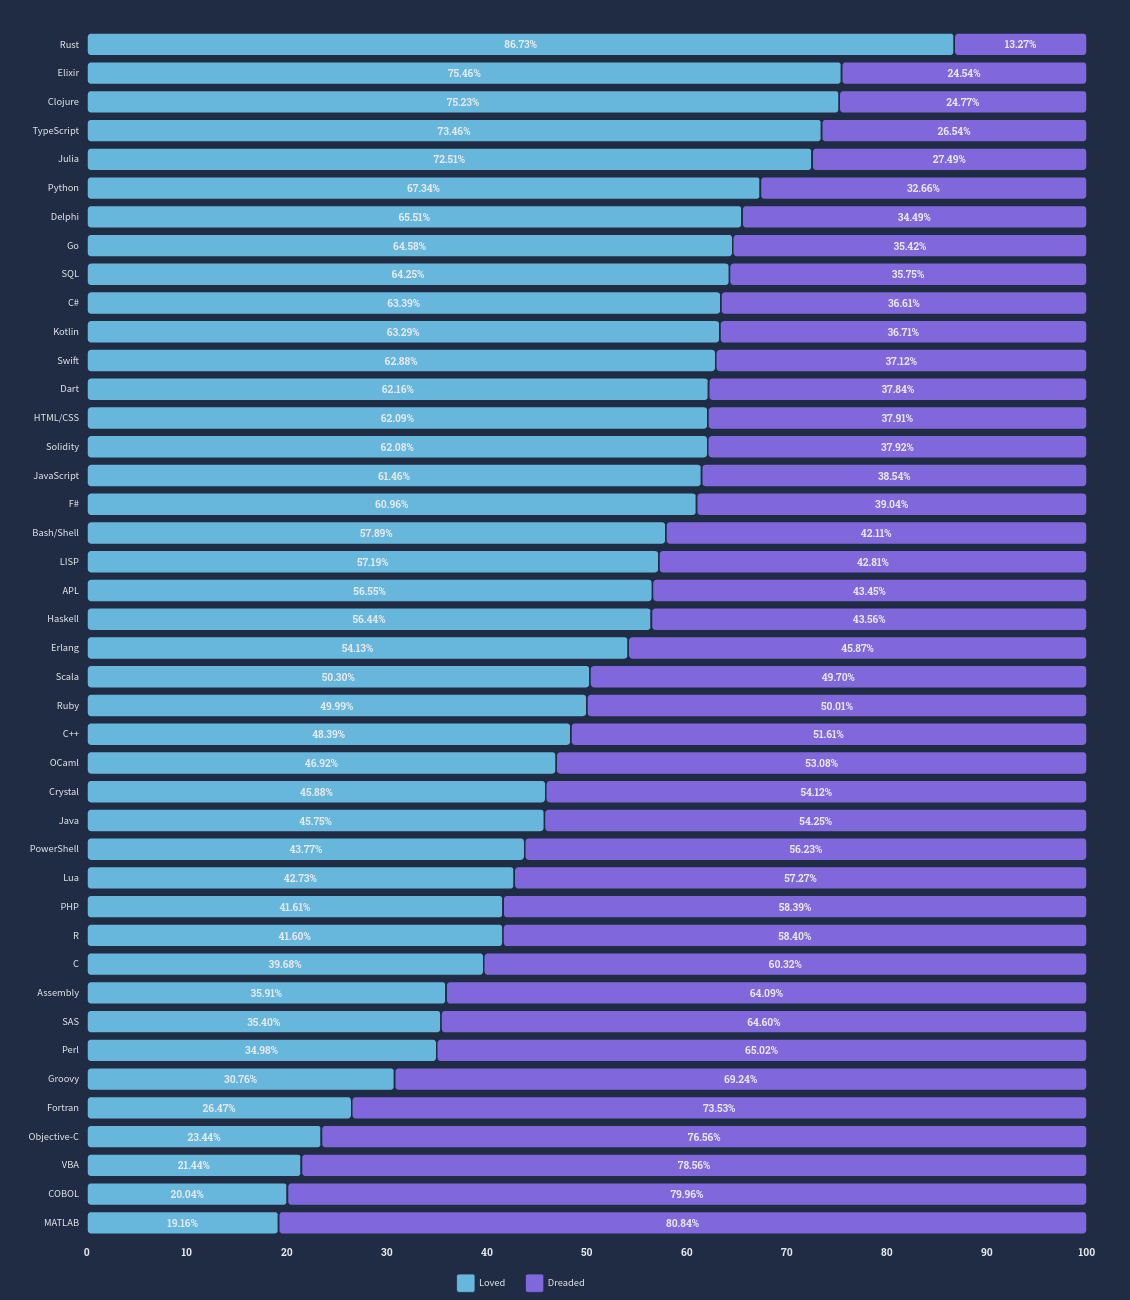
\includegraphics[width=\textwidth]{stack_loved}
  \caption{Wykres przedstawiający współczynnik uwielbiania/nienawiści danej technologii}
  \label{stack:loved}
  \caption*{Źródło: \url{https://survey.stackoverflow.co/2022}}
\end{figure}
\FloatBarrier

\subsection*{Yew}
Yew to framework umożliwiający tworzenie witryn WWW w języku Rust.
Z użyciem tej biblioteki możliwe jest konstruowanie niezawodnych
oraz wydajnych stron internetowych. Yew wykorzystuje WebAssembly wraz
z renderowaniem po stronie serwera, aby znacznie przyśpieszyć działanie
aplikacji na docelowej platformie. Umożliwia również na wykorzystanie 
funkcjonalności innych popularnych języków wykorzystywanych do tworzenia
aplikacji webowych takich jak JavaScript poprzez wykorzystanie biblioteki
wasm-bindgen udostępniającej standardową funkcjonalność tego języka oraz
pozwalającą na połączenie ze skryptami stworzonymi w tym języku.

Do tworzenia stron Yew wykorzystuje język podobny do HTML i JSX dzięki
czemu jest przystępny dla programistów mających wcześniejsze doświadczenie
z tymi technologiami. Podobnie jak inne środowiska takie jak React czy Angular
tworzone są komponenty, które mogą być wielokrotnie używane w różnych komponentach
oraz podstronach co sprawia, że kod jest czytelniejszy, zmniejszona jest jego złożoność
oraz możliwe jest wyeliminowanie niepotrzebnych powtórzeń.

\subsection*{Bootstrap}
Bootstrap to darmowe i otwarto-źródłowe środowisko programistyczne składające się
ze zbioru szablonów stworzonych w językach HTML, CSS i JavaScript, które mogą
być dowolnie wykorzystane z kompatybilnymi technologiami.
Ten framework zawiera podstawowe style potrzebne, aby stworzyć responsywną 
aplikacje webowe na wielu urządzeniach z różnymi rozmiarami ekranów oraz rozdzielczością. 

\subsection*{TypeScript}
TypeScript to darmowy, otwarto źródłowy stworzony oraz utrzymywane przez przedsiębiorstow Microsoft.
Jest rozszerzeniem popularnego języka JavaScript dodającym szeroko zastosowane funkcjonalności
w innych statycznie typowanych językach, tj. adnotacje typów oraz ich sprawdzanie
podczas kompilacji, interfejsy, typy wyliczeniowe czy uogólnienia.
Dodatkowo rozszerza język o słowa kluczowe async/await ułatwiające pracę
z asynchronicznymi funkcjami. Język TypeScript jest całkowicie kompatybilny ze 
środowiskami wspierającymi JavaScript - jest to język transpilowany do JS, a
dodatkowe funkcjonalności dostępne są jedynie podczas tworzenia oprogramowania.

Jego wykorzystanie w aplikacji zostało ograniczone jedynie do wykonania funkcjonalności,
których implementacja w pozostałych technologiach była niemożliwa lub znacznie 
utrudniona. Są to głównie funkcje pomocnicze wywoływane w odpowiednich komponentach
stworzonych w technologii Yew.

\section{Aplikacja serwerowa}

\subsection*{.NET Core}
.NET Core to następca popularnej platformy programistycznej .NET Framework stworzonej przez
firmę Microsoft. W przeciwieństwie do poprzednika, którego oficjalne wsparcie ograniczone było
do systemu Windows, a same oprogramowanie było własnościowe, jest to technologia otwarto-źródłowa
wspierająca wiele systemów operacyjnych \cite{price2021c}. Możliwe jest to poprzez zastosowanie
języka pośredniego niezależnego od systemu lub sprzętu. Instrukcje te tłumaczone są w 
wirtualnej maszynie CLR (ang. \textit{Common Language Runtime}) na język maszynowy, a
następnie wykonywane jak standardowy natywny kod \cite{msdn:clr}. Dzięki takiemu podjeściu
możliwe jest wytworzenie przenośnego oprogramowania, które może być wykorzystane na wielu
systemach.

\subsection*{C\#}
C\# to silnie typowany język obiektowy wysokiego poziomu stworzony przez firmę Microsoft.
Do kompilacji wykorzystywane jest środowisko .NET, dzięki czemu zachowane są
jego cechy takie jak przenośność oprogramowania oraz możliwość wykorzystania
innych języków programowania bazujących na tej technologii.

Dzięki automatycznemu zarządzaniu pamięcią ułatwia znacznie tworzenie
oprogramowania, gdyż w bezpiecznym kontekście nie pozwala na 
błędne jej wykorzystanie. Wykonywane jest to poprzez zastosowanie
mechanizmu odśmiecania pamięci (ang. \textit{garbage collection}).

C\# zawiera również rozszerzenia kolekcji LINQ (ang. \textit{Language Integrated Query})
pozwalające na wykonywanie na nich dodatkowych operacji, tj. grupowanie, sortowanie czy wyszukiwanie.
Te dodatkowe metody mogą być wykorzystane do działań na róznych źródłach danych takich jak dokumenty XML
czy też bazy danych SQL \cite{zhang2014}. Ich wysokopoziomowy kod jest przenośny i może być
wykorzystywany w takiej samej formie przy różnych źródłach danych.

Kolejną zaletą tej technologii jest możliwość wykorzystania meta-programowania. 
Jest to technika umożliwiająca modyfikację kodu podczas jego kompilacji lub wykonywania. 
Dzięki niej podczas wykonywania programu, poprzez refleksję, możliwe jest rozpoznanie
typu obiektu oraz jego modyfikacja. Pozwala również na tworzenie drzew wyrażeń, które
mogą zostać dynamicznie skompilowane w celu, np. wykorzystania zaawansowanej logiki
biznesowej, która może być zmienna.

\subsection*{ASP.NET}
ASP.NET to modularna platforma programistyczna oparta na technologii .NET. 
Jej bogata funkcjonalność pozwala na tworzenie stron internetowych, API HTTP oraz 
wiele innych aplikacji webowych poprzez zastosowanie wielu z jej rozszerzeń.
Jednym z nich jest wstrzykiwanie zależności (ang. \textit{dependency injection})
pozwalające na uzyskanie rozwiązania podobnego do wzorca architektury inwersji
kontroli (ang. \textit{Inversion of Control}). W takiej architekturze, zamiast
polegać na szczegółowej implementacji danej funkcjonalności czy serwisu,
użytkownik otrzymuje interfejs mówiący jedynie o tym do czego jest on przeznaczony.
Dzięki temu uzyskany kod jest całkowicie oddzielny od implementacji i pozwala
na znaczne ograniczenie efektów ubocznych przy działaniach takich jak refaktoryzacja,
restrukturyzacja czy przenoszenie implementacji, aby ta korzystały z innej biblioteki, np.
przy zmianie systemu bazodanowego.

Poprzez zastosowanie tak zwanych pośredników (ang. \textit{Middleware}) ASP.NET udostępnia
bardzo modularną oraz modyfikowalną strukturę przetwarzania zapytań HTTP.
Są to proste kroki, w których wykonywana jest logika związana z zapytaniem lub odpowiedzią
wysyłaną przez serwer. Podczas ich wykonania możliwy jest dostęp do danych zawartych
w zapytania oraz następnie jego modyfikacja, jak również decyzja o tym czy powinno
być ono propagowane do dalszych warstw. Przydatne to jest w przypadku, np. autoryzacji
gdzie w module sprawdzającym tożsamość użytkownika możliwe jest modyfikacja oraz zwrócenie
odpowiedzi o nieautoryzowanym dostępie i nie przekazywanie zapytania dalej do warstw, które zajmują
się dostępem do danych. Możliwe jest również zastosowanie innych pośredników takich
jak przechowywanie zapytań oraz odpowiedzi na nie w pamięci podręcznej, co znacznie
zwiększa wydajność systemu przy wielu takich samych zapytaniach. Poza wieloma wbudowanymi
pośrednikami programista sam może definiować swoją własną logikę oraz umieszczać
ją w odpowiednim momencie łańcucha wykonania.

\subsection*{MongoDB}
MongoDB to wieloplatformowy system bazodanowy. Dane przechowywane są w postaci dokumentów,
w formacie podobnym do JSON (ang. \textit{JavaScript Object Notation}), określaną nazwą
BSON (ang. \textit{Binary JSON}). Główną różnicą między tymi formatami jest sposób kodowania
danych - w przypadku formatu JSON jest to postać znaków UTF-8, a BSON jest to zapis binarny.
Pozwala to na łatwą konwersję między tymi typami, czyli co za tym idzie również uzyskiwanie
czytelnych dla człowieka danych, tym samym oszczędzając miejsce potrzebne do przechowywania
informacji jak również przyśpieszenie niektórych operacji jak indeksowanie.

W porównaniu do klasycznych baz danych SQL, MongoDB pozwala na większą elastyczność dzięki braku
konieczności określania schematu tabel. Wszystkie schematy są dynamiczne i mogą w dowolnym momencie 
zostać zmienione w celu dodania dodatkowych informacji jednocześnie nie zmieniając pozostałych
danych zapisanych w danej kolekcji. Jednocześnie ten system pozwala na tworzenie 
walidatorów kolekcji, co przydaje się w momentach kiedy chcemy uzyskać większą kontrolę
nad strukturą danych.

\subsection*{Docker}
Docker to zbiór oprogramowania umożliwiający dystrybucję oprogramowania jako tzw. kontener.
Są to wyspecjalizowane maszyny wirtualne, zawierające jedynie oprogramowanie potrzebne
do uruchomienia danego rozwiązania. Podobnie jak zwykłe rozwiązania wirtualizacyjne
są one od siebie odizolowane, ale w przeciwieństwie do innych, klasycznych rozwiązań
działają one na tym samym jądrze systemu operacyjnego dzięki czemu zużywają znacznie
mniej zasobów\cite{docker:what_is_container}. Odpowiednio skonfigurowane połączenia
między maszynami umożliwiają komunikację, np. poprzez protokół TCP. 
Po odpowiednim spakowaniu obrazu ta technologia umożliwia wykorzystanie identycznego
oprogramowania w różnych środowiskach niezależnie od systemu operacyjnego hosta.

Oprogramowaniem, które wchodzi w skład tego kompleksu i zostało ekstensywnie wykorzystane 
w realizacji projektu jest docker-compose. Te narzędzie wykorzystuje pliki konfiguracyjne
w formacie YAML, aby ułatwić pracę w środowiskach wymagających użycia kliku kontenerów, np.
w przypadku aplikacji serwerowej, która ma komunikować się z bazą danych.

\section{Urządzenie pomiarowe}
Urządzenie pomiarowe wykonane zostało na płytce Raspberry Pi Pico W, do którego z wykorzystaniem
portów ogólnego przeznaczenia GPIO podłączono sensory badające parametry środowiska.

\subsection*{Raspberry Pi Pico W}
Raspberry Pi Pico W to komputer jedno-płytkowy zbudowany na podstawie mikrokontrolera RP2040. 
Do głównych jego cech, które zostały wykorzystane do stworzenia systemu należą \cite{rp2040:datasheet}:
\begin{itemize}
  \item procesor dwurdzeniowy ARM Cortex-M0+,
  \item 264kB pamięci SRAM,
  \item 2MB pamięci flash,
  \item kontroller DMA (ang. \textit{Direct memory access}),
  \item 30 pinów GPIO (ang. \textit{General-purpose input/output}),
  \item 2 kontrollery SPI (ang. \textit{Direct memory access}),
  \item 2 kontrollery I2C (ang. \textit{Serial Peripheral Interface}),
  \item 16 kanałów PWM (ang. \textit{Pulse-width modulation}).
\end{itemize}
Płytka umożliwia łączność z siecią Wi-Fi przy użyciu wbudowanego chipu CYW43439
obsługujący standard 802.11n, który w odpowiednich warunkach pozwala na łączność
z prędkością do 600Mb/s. Wraz z nowszymi wersjami SDK umożliwia również wykorzystanie
całego potencjału tego urządzenia i umożliwia na połączenia protokołem Bluetooth.

Aktualnie dostępne oprogramowanie pozwala tworzyć systemy w językach programowania takich jak
Assembly, C, C++, Python oraz Rust. Istnieje również nieoficjalne wsparcie dla środowiska
Arduino oraz możliwość wykorzystania istniejących na tą platformę bibliotek.
Ze względu na język, w którym utworzono SDK (ang. \textit{Software Development Kit}) dla
tej platformy (język programowania C), najczęściej wykorzystywane są języki C oraz C++
ze względu na wysoki stopień kompatybilności.

\subsection*{C++}
C++ to obiektowy język programowania wysokiego poziomu, będący często określany jako
rozszerzenie języka C często używanego do tworzenia oprogramowania na systemy wbudowane.
Obsługuje on wysokopoziomowe abstrakcje takie jak obiekty, programowanie generyczne czy
abstrakcje pozwalając w tym samym czasie na używanie niskopoziomowej funkcjonalności 
takiej jak zarządzenie pamięcią czy dostęp do rejestrów procesora oraz używanie języka asembler.
Przez te cechy używany jest tam, gdzie potrzebna jest wysoka wydajność lub zasoby komputerowe
są znacznie ograniczone, np. serwery WWW, gry komputerowe czy systemy wbudowane.

W porównaniu do C zawiera również rozbudowaną standardową bibliotekę klas i funkcji.
Dodaje ona dodatkową funkcjonalność taką jak zaawansowane typy pozwalające na
przechowywanie zmiennej liczby danych, algorytmy takie jak sortowanie czy 
generowanie liczb losowych, obsługa plików, czasu oraz wielowątkowości.

\chapter{Projekt i implementacja}
W tym rozdziale przedstawiono szczegóły implementacji systemu. 
Poszczególne zagadnienia oraz aplikacje wchodzące w jego skład
zostały opisane w oddzielnych sekcjach tego rozdziału.

\section{Komponenty systemu i komunikacja}
Komunikacja między komponentami aplikacji odbywa się z wykorzystaniem protokołu 
HTTP (ang. \textit{Hypertext Transfer Protocol}).
Jest to jedna z technologii wykorzystywana w modelu TCP/IP 
nazywanego również protokołem Internetowym (ang. \textit{Internet Protocol}).
Jest protokołem bezstanowym \cite{http:rfc9110} służącym do przesyłania
informacji w postaci hipertekstowej i jest podstawowym rozwiązaniem
stosowanym w sieci WWW (ang. \textit{World Wide Web}), będąca systemem 
służącym do udostępniania informacji poprzez sieć Internet
z wykorzystaniem adresów URI (ang. \textit{Uniform Resource Identifier}) \cite{Jacobs:04:AWW}.

Dodatkowo wykorzystany został protokół kanałów komunikacyjnych WebSocket.
Pracują one w trybie pełnego dupleksu, co zezwala na obustronną komunikację
klienta z serwerem oraz serwera z klientem. Największą jego zaletą jest
możliwość wykorzystania protokołu HTTP w celu ustanowienia połączenia 
oraz wykorzystanie tych samych portów 80 oraz 443.
Aby ustanowić połączenie klient powinien wysłać odpowiedni
nagłówek nazywany HTTP Upgrade, na który serwer odpowiada z informacją o zmianie protokołu.
Następnie połączenie zmienia protokół z HTTP do binarnej transmisji bezpośrednio wykorzystującej TCP.
W tym momencie obie strony z jego wykorzystaniem mogą odczytywać oraz wysyłać wiadomości
pomiędzy sobą.

Protokoły wykorzystane w celu komunikacji przedstawione zostały na Rys. \ref{diagram:comms}.
\begin{figure}[h!]
  \centering
  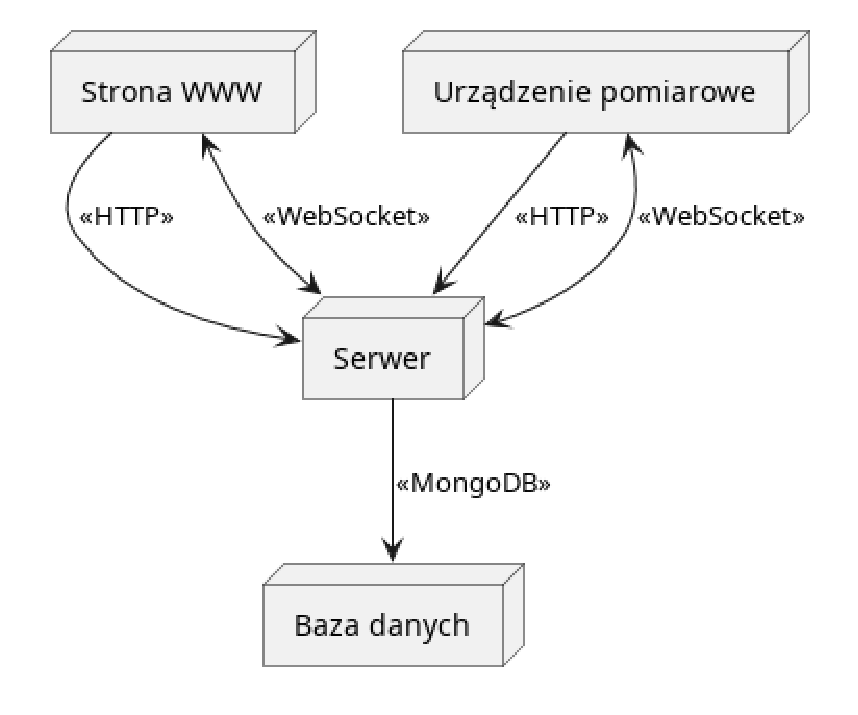
\includegraphics[width=\textwidth]{comms_diagram}
  \caption{Protokoły wykorzystane w komunikacji między komponentami}
  \label{diagram:comms}
\end{figure}

\section{Aplikacja serwerowa}
Aplikacja serwerowa została zaimplementowana jako centralny komponent systemu.
Zajmuje się zapisem odczytów w bazie danych, przetwarzaniem zapytań
pozostałych warstw, klienckiej oraz urządzeń pomiarowych,
poprzez wykorzystanie różnych metod HTTP.
Metoda POST zajmuje używana jest w nim do przekazywania danych
dla serwera w procesach takich jak tworzenie konta użytkownika,
wysyłanie nowego odczytu czy uwierzytelnianie.
Aplikacja następnie przetwarza te zapytanie oraz w odpowiedni 
sposób na nie reaguje, np. zapisując je na stałe do bazy danych 
lub wysyłając notyfikację użytkownikowi, po czym odpowiada
odpowiednim statusem klientowi.
Kolejną szeroko zastosowaną metodą jest GET. Służy ona do pobierania
zasobów z serwera. Klient wykorzystuje odpowiedni adres URI z
podstawowymi danymi lub bez, pod który wykonuje zapytanie, a
następnie serwer zwraca odpowiedź z zażądanymi informacjami.
Metodami służącymi do modyfikacji zasobów są PUT oraz DELETE.
Pierwsza z nich wykorzystywana jest do zmieniania istniejących
już zasobów lub tworzenia ich na nowo. DELETE natomiast służy
do usuwania zasobów.

\subsection{Architektura aplikacji}
Jako szkielet logiki aplikacji został wykorzystany wzorzec CQRS 
(ang. \textit{Command Query Responsibility Separation}).
W tym modelu akcje dzielą się na dwa typy komendy oraz zapytania \cite{fowler:cqrs}.
Komendy służą do interakcji z systemem, np. tworzenie użytkowników.
Mogą zawierać dodatkową logikę jak weryfikacja danych wejściowych 
czy sprawdzanie duplikatów.
Zapytania spełniają funkcję dostępu do danych. Pobierane oraz
filtrowane są w nich informacje z systemu i w razie potrzeby
odpowiednio transformowane.
Dzięki stosowaniu się do zasad tej metodyki aplikacja wolna
jest od efektów ubocznych i tworzenie zapytań nie zmienia
wartości systemu. Pozwala również na uproszczenie logiki
aplikacji ze względu na podział na proste moduły oraz bardzo
dobrą skalowalność z rozwiązaniami wielowątkowymi.
W implementacji tej metodyki wykorzystano bibliotekę MediatR.
Udostępnia ona bardzo łatwy w użyciu wzorzec mediatora.
Pozwala on na redukcję zależności między komponentami poprzez
zastosowanie centralnego obiektu zajmującego się komunikacją między nimi\cite{freeman2004head}.
W tym przypadku komponentami są komendy oraz zapytania i do ich realizacji
została wykorzystana dynamiczna implementacja centralnego
mediatora z biblioteki MediatR. Oddziela to dane od implementacji
zachowań i pozwala na ich niezależną modyfikacje.

Klasy danych wywodzą się z głównej klasy abstrakcyjnej \textbf{BaseModel}.
Zawiera ona podstawowe dane o obiekcie tj. id, data stworzenia oraz data modyfikacji.
Poza tym implementuje podstawowe funkcje do porównywania z innymi obiektami oraz
tworzeniu kodu hash. Bezpośrednio z niej dziedziczy klasa \textbf{Reading} odpowiadająca
za przechowywanie szczegółów o odczytach. Zawiera informacje o typie odczytu, jego wartości,
dacie i czasie kiedy dany odczyt został pobrany oraz jego jednosce.
Dodatkową klasą abstrakcyjną, która sama dziedziczy po klasie \textbf{BaseModel} i
jest wykorzystywana przez inne klasy domeny jest \textbf{BaseUser}. Jest to bazowa klasa
użytkownika i zawiera informacje takie jak nazwa użytkownika, zakodowane hasło, stan aktywności
oraz rola. Z tej klasy dziedziczą klasy \textbf{Device} oraz \textbf{User}. Pierwsza z nich 
zawiera dodatkowe informacje o urządzeniach pomiarowych, a druga o użytkownikach lub administratorach 
w zależności od ich roli.
Oddzielnym modelem jest klasa służąca do przechowywania konfiguracji. Składa się ona z dwóch pól -
klucza oraz wartości. Wartość nie ma z góry określonego typu i może być dowolnym obiektem, który
jest możliwy do zapisu w postaci JSON.
Zależności między klasami zostały przedstawione na Rys. \ref{diagram:domain}.
\begin{figure}[h!]
  \centering
  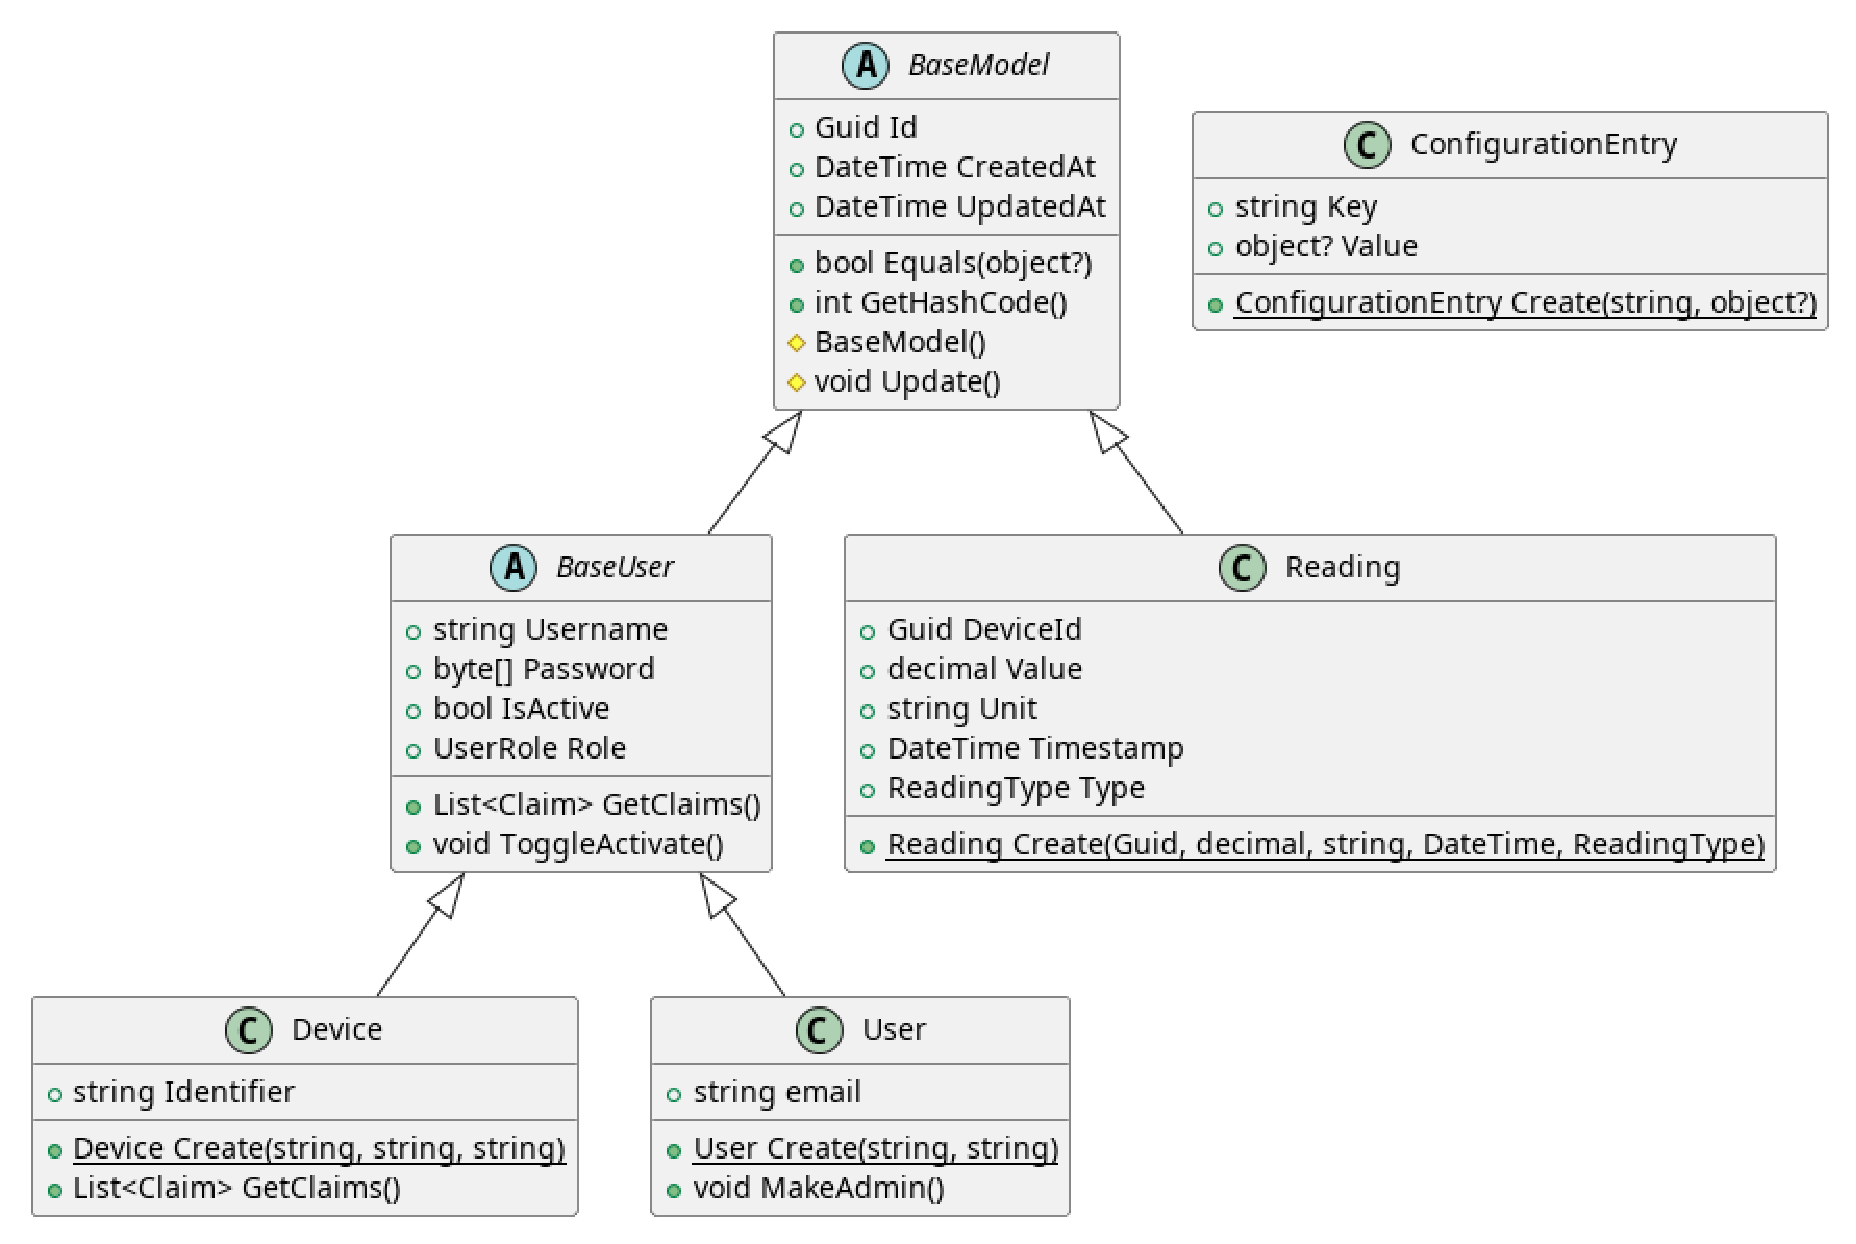
\includegraphics[width=\textwidth]{domain}
  \caption{Diagram klas modeli danych}
  \label{diagram:domain}
\end{figure}

Serwis notyfikacji został zaimplementowany z użyciem wzorca dekorator.
Jest to wzorzec projektowy pozwalający na dynamiczne dodawanie nowego
zachowania obiektowi bez modyfikacji innych obiektów tej samej klasy
\cite{freeman2004head}. Tym samym ułatwia on dostosowanie się do zasady
pojedynczej odpowiedzialności (ang. \textit{Single responsibility principle})
poprzez wydzielenie logiki na klasy zajmujące się tylko jednym zadaniem.
Jego wykorzystanie oznacza również zastosowanie zasady otwarte-zamknięte, w
której części systemu powinny być otwarte na rozszerzanie, ale zamknięte
na modyfikacje \cite{meyer1988object}. Jest to możliwe, gdyż dekorator pozwala
na dodanie nowych funkcjonalności obiektowi bez jego ponownego tworzenia.
Z jego wykorzystaniem użytkownik jest w stanie skonfigurować system notyfikacji,
aby ten wysyłał powiadomienia do różnych celów takich jak poczta elektroniczna
czy powiadomienia z wykorzystaniem połączeń WebSocket. Wzorzec dekorator został
przedstawiony za pomocą diagramu klas na Rys. \ref{pattern:decorator}.
\begin{figure}[h!]
  \centering
  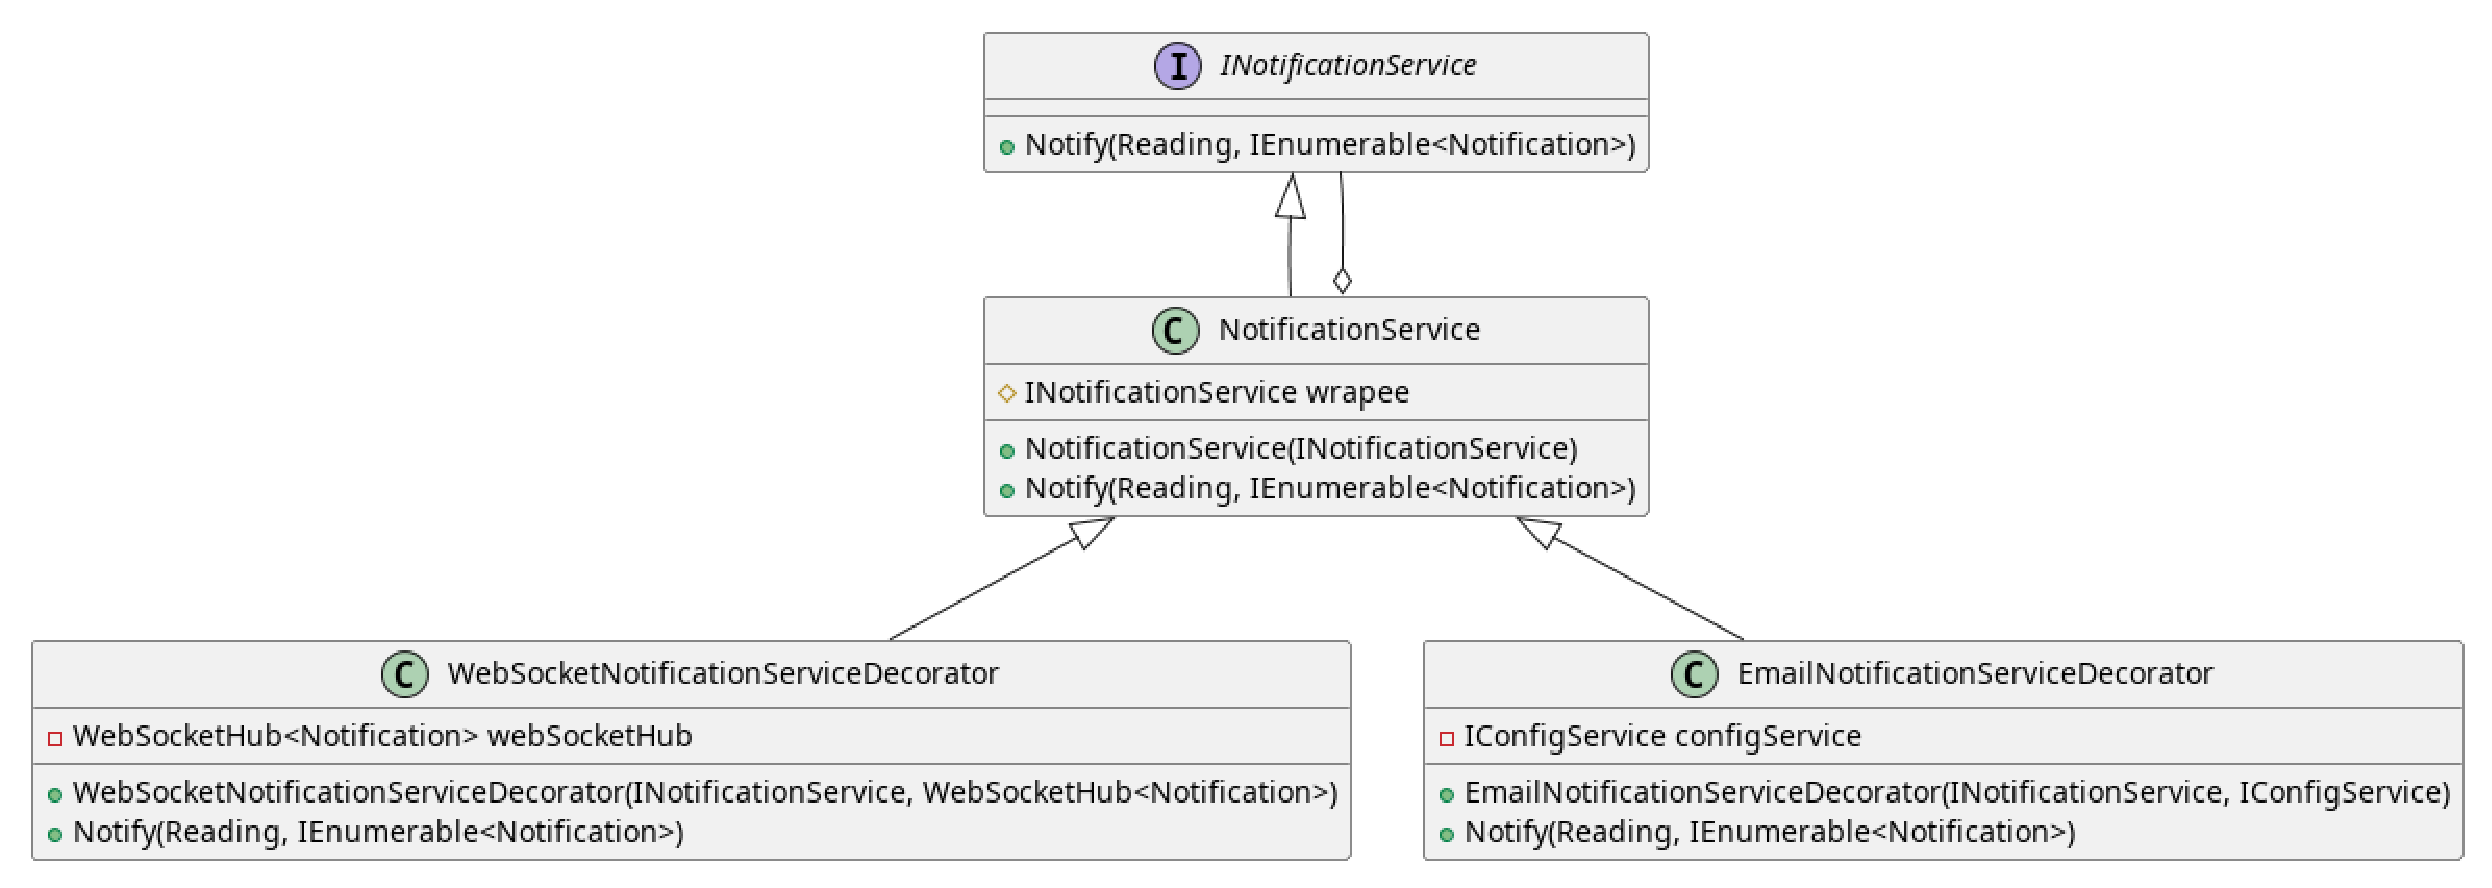
\includegraphics[width=\textwidth]{decorator}
  \caption{Diagram klas wzorca dekorator}
  \label{pattern:decorator}
\end{figure}

Pozostałe aplikacje w systemie mogą komunikować się z serwerem poprzez wykorzystanie
zapytań do odpowiednich kontrolerów. Zależnie od punktu końcowego muszą one
przesłać odpowiednie informacje w postaci ciała, ciągu lub argumentu pozycyjnego
zapytania. Aplikacja zawiera kontrolery zajmujące się odpowiednim im zadaniom:
\begin{itemize}
  \item zapis oraz odczyt parametrów środowiska,
  \item autoryzacja oraz tworzenie kont,
  \item konfiguracja oraz pobieranie konfiguracji systemu,
  \item pobieranie szczegółowych danych o urządzeniach oraz ich statusie,
  \item rozpoczynanie połączenia z WebSocket'ami.
\end{itemize}
W celu ułatwienia obsługi każdy z kontrolerów znajduje się na ścieżce URI odpowiadającej
jego nazwie, np. kontroler odczytów znajduje się pod ścieżką /api/Reading.
Dodatkowo serwer udostępnia dwa połączenia WebSocket - notyfikacyjne oraz
dla urządzeń. Pierwsze z gniazd wykorzystywane jest do przesyłania
powiadomień do pozostałych aplikacji. Autoryzowani użytkownicy mogą
się z nim połączyć, aby uzyskać dostęp do wiadomości o niespodziewanych
wartościach odczytów parametrów środowiska. Gniazdo przeznaczone dla
urządzeń służy natomiast do synchronizacji konfiguracji oraz
udostępnienia statusu. Wszystkie połączenia powinny co 30 sekund
wysyłać wiadomość z zawartością "ping", aby zapewnić stałość połączenia.
W przeciwnym wypadku serwer uznaje połączenie za przerwane i zamyka je.
Wykorzystywane są one również do udostępniania notyfikacji oraz
synchronizacji konfiguracji z pozostałymi urządzeniami.
Diagram klas zawierający informacje o kontrolerach został przedstawiony na
Rys. \ref{diagram:controller_class}.
\begin{figure}[h!]
  \centering
  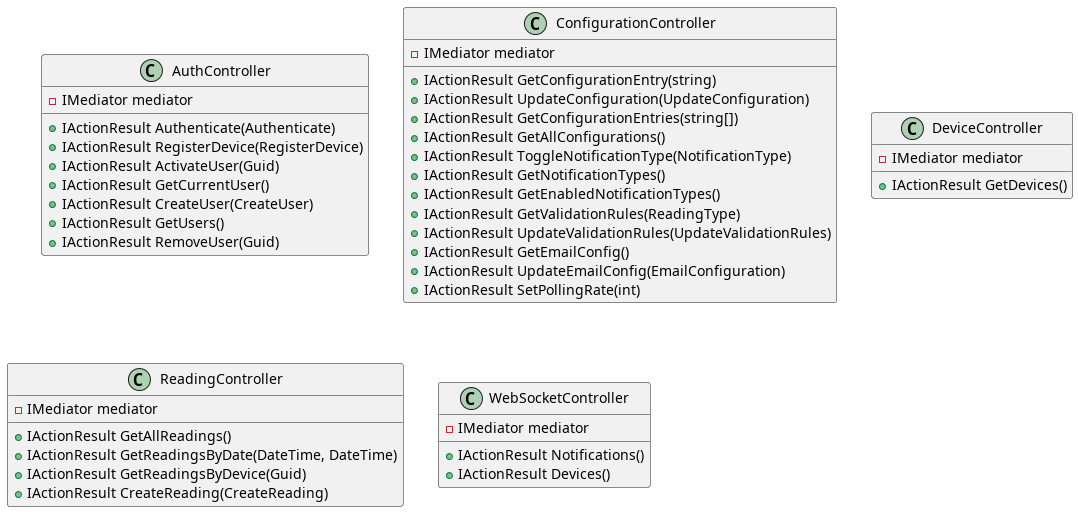
\includegraphics[width=\textwidth]{controller_class}
  \caption{Diagram klas kontrolerów}
  \label{diagram:controller_class}
\end{figure}

Dostęp do danych odbywa się poprzez wykorzystanie oficjalnego sterownik
baz danych MongoDB dla środowiska .NET. Jego wykorzystanie 
umożliwiło na prostą interakcję między aplikacją oraz bazą
danych. Zamiast ręcznie dokonywać połączenia oraz przesyłać
komendy możliwa jest interakcja poprzez udostępniony interfejs.
Umożliwia on na wykorzystanie zaawansowanych technik takich jak
LINQ co znacznie ułatwiło tworzenie zapytań. Technologia ta
pomaga również w mapowaniu obiektów baz danych na klasy języka C\#.
W większości przypadków takie zależności tworzone są automatycznie,
jedynie w przypadku nadmiarowych lub braku wymaganych danych potrzebna
jest interakcja programisty. Przykładem z implementacji jest wymaganie
mapowania klas dziedziczących.
\begin{lstlisting}[language={[Sharp]C},caption={Tworzenie mapy klas dla typów użytkownika},label={mongodb:user},captionpos=b]
BsonClassMap.RegisterClassMap<BaseUser>(cm =>
{
    cm.AutoMap();
    cm.AddKnownType(typeof(Device));
    cm.AddKnownType(typeof(User));
});
\end{lstlisting}
W listingu \ref{mongodb:user} tworzona jest mapa automatyczna dla klasy BaseUser - podstawowej
użytkownika, a następnie wiązane są z nią dwa typy pochodne - Device, czyli urządzenie
oraz User, czyli użytkownik. Pozwala to na dostęp do obu typów użytkownika
z jednego kontekstu bazy danych.


\subsection{Implementacja wybranych funkcjonalności}

Wykorzystanie technologii ASP.NET ułatwiło znacznie wykonanie systemu autoryzacji. 
Pakiet Microsoft.AspNetCore.Authentication zawiera często wykorzystywane metody
uwierzytelniania użytkowników. W implementacji aplikacji użyto metody tokenów JWT
(ang. \textit{JSON Web Token}). Jest to krótka, zakodowana w systemie Base64, 
reprezentacja uprawnień użytkownika używana w środowiskach z ograniczoną przestrzenią 
takich jak HTTP\cite{jwt:rfc7519}. Oprócz tego zawiera informacje o
czasie jego przedawnienia, audiencji oraz emitenta. Dzięki temu
może zostać wykorzystany w systemach pojedynczego logowania
SSO (ang. \textit{Single sign-on}) i wykorzystywany poprzez wiele aplikacji.
W implementacji został wykorzystany algorytm HmacSha256 do cyfrowego
podpisywania ważności tokenu. Sterowanie innymi parametrami takimi jak czas
przedawnienia, audiencja orz emitent odbywa się za pomocą edytowalnych
plików konfiguracyjnych.
\begin{lstlisting}[language={[Sharp]C},caption={Tworzenie tokenu JWT},label={jwt:create},captionpos=b]
var token = new JwtSecurityToken(
  config["Issuer"],
  config["Audience"],
  claims,
  expires: DateTime.Now.Add(expiration),
  signingCredentials: new SigningCredentials(
    new SymmetricSecurityKey(Encoding.UTF8.GetBytes(config["SecretKey"])),
  SecurityAlgorithms.HmacSha256));
\end{lstlisting} 
Następnie w konfiguracji aplikacji umieszczono odpowiednie opcje walidacji tokenów.
Ich konfiguracja została zaprezentowana na listingu \ref{jwt:opts}.
\begin{lstlisting}[language={[Sharp]C},caption={Opcje walidacji JWT},label={jwt:opts},captionpos=b]
opt.TokenValidationParameters = new TokenValidationParameters
{
  ValidateIssuer = true,
  ValidIssuer = config.GetValue<string>("Issuer"),
  ValidateAudience = true,
  ValidAudience = config.GetValue<string>("Audience"),
  ValidateLifetime = true,
  ClockSkew = TimeSpan.FromSeconds(0),
  ValidateIssuerSigningKey = true,
  IssuerSigningKey = new SymmetricSecurityKey(
    Encoding.UTF8.GetBytes(config.GetValue<string>("SecretKey"))
  )
};
\end{lstlisting} 
Ustawione zostały opcje takie jak walidacja emitenta, audiencji, czasu życia oraz
klucza, którym został podpisany token.
Hasła użytkowników przechowywane są po wcześniejszym zakodowaniu algorytmem SHA256
z dodatkowymi informacjami nazywanymi solą. Są to losowe dane, które pozwalają na
dodatkowe zabezpieczenie kluczy przed wykryciem duplikatów lub ataków słownikowych
\cite{anderson2020security}.
Aby odpowiednio przejść proces uwierzytelniania użytkownik musi przesłać
swoją nazwę użytkownika oraz hasło zapytaniem z metodą POST pod odpowiedni adres
URI. Następnie jeżeli dane są prawidłowe w odpowiedzi otrzyma on wartość
token, która następnie może wykorzystać do dostępu do zablokowanych anonimowym
użytkownikom zasobów, takich jak tworzenie nowych odczytów. Wartość
ta musi zostać przesłana w nagłówku Authorization.
Użytkownicy dzielą się na różne role: administrator, użytkownik oraz urządzenie.
Administrator ma dostęp do wszystkich opcji aplikacji - konfiguracji, zarządzania odczytami
oraz użytkownikami, przeglądanie zasobów. Urządzenie może zarządzać jedynie swoimi
danymi, a zwykły użytkownik nie ma dostępu do edycji zasobów i może jedynie przeglądać
wartości.

Reguły sterujące logiką wysyłania powiadomień zbudowane zostały przy użyciu systemu
ekspresji środowiska .NET. Dzięki temu użytkownik może w rozbudowany sposób
tworzyć logikę określającą przy jakich warunkach powinna być wysłana dana wiadomość.
Dzięki temu, że są one kompilowane podczas wykonywania programu mogą przyjąć dowolną
formę, więc nie ograniczają użytkownika w ich tworzeniu oraz modyfikacji.
\begin{lstlisting}[language={[Sharp]C},caption={Kompilacja formy tekstowej ekspresji},label={valid:comp},captionpos=b]
try
{
    var options = ScriptOptions.Default.AddReferences(typeof(Reading).Assembly);
    var expression = await CSharpScript.EvaluateAsync<Expression<Func<Reading, bool>>>(
        rule.Condition,
        options
    );
    newRules.Add(
        new ValidationRule
        {
            Condition = expression,
            Message = rule.Message,
            Severity = rule.Severity
        }
    );
}
catch (CompilationErrorException e)
{
    throw new InvalidRuleException(e.Message.Split(": ").Last());
}
\end{lstlisting}
Na listingu \ref{valid:comp} przedstawiono kod odpowiedzialny za kompilację ekspresji podczas działania
aplikacji. Wykorzystana została do tego biblioteka Microsoft.CodeAnalysis. Ekspresja kompilowana jest
jako funkcja przyjmująca na wejściu odczyt oraz zwracająca wartość bool. W przypadku nieodpowiedniej składni
łapany jest błąd kompilacji a następnie zwracana jest on nim informacja użytkownikowi.
Serializacja oraz de-serializacja ekspresji została wykonana przy użyciu biblioteki
Remote.Linq pozwalająca na ich zapis oraz odczyt do różnych formatów takich jak
JSON czy XML, które następnie przechowywane są w bazie danych. Aby wykorzystać ją
z bazą danych MongoDB należało zaimplementować dodatkowy serializator, którego implementacja
została przedstawiona na listingu \ref{expr:serialization}.
\begin{lstlisting}[language={[Sharp]C},caption={Serializacja ekspresji},label={expr:serialization},captionpos=b]
public Expression<TDelegate> Deserialize(
    BsonDeserializationContext context,
    BsonDeserializationArgs args
)
{
    var bsonReader = context.Reader;
    if (bsonReader.CurrentBsonType == BsonType.Null)
    {
        bsonReader.ReadNull();
        return null;
    }
    var binaryData = bsonReader.ReadBinaryData();
    var remote = JsonSerializer.Deserialize<Remote.Linq.Expressions.LambdaExpression>(
        binaryData.Bytes,
        jsonSerializerOptions
    );
    return (Expression<TDelegate>)remote.ToLinqExpression();
}
public void Serialize(
    BsonSerializationContext context,
    BsonSerializationArgs args,
    Expression<TDelegate> value
)
{
    var bsonWriter = context.Writer;
    if (value is null)
    {
        bsonWriter.WriteNull();
        return;
    }
    var remote = value.ToRemoteLinqExpression();
    bsonWriter.WriteBinaryData(
        JsonSerializer.SerializeToUtf8Bytes(remote, jsonSerializerOptions)
    );
}
\end{lstlisting}

Aby ułatwić implementację pozostałych aplikacji oraz w celu zapewnienia dokumentacji
wykorzystano bibliotekę Swashbuckle. Dostarcza ona składniki takie jak 
\begin{itemize}
  \item generator schematów OpenAPI, które mogą być następnie wykorzystane do generowania klientów
wykorzystujących dane API,
  \item generator dokumentacji bazujący na komentarzach znajdujących się w kodzie aplikacji,
  \item interfejs swagger-ui umożliwiający na przeglądanie zasobów z poziomu przeglądarki internetowej.
\end{itemize}
Interfejs swagger-ui przedstawiono na Rys. \ref{swagger:interface}.
\begin{figure}[h!]
  \centering
  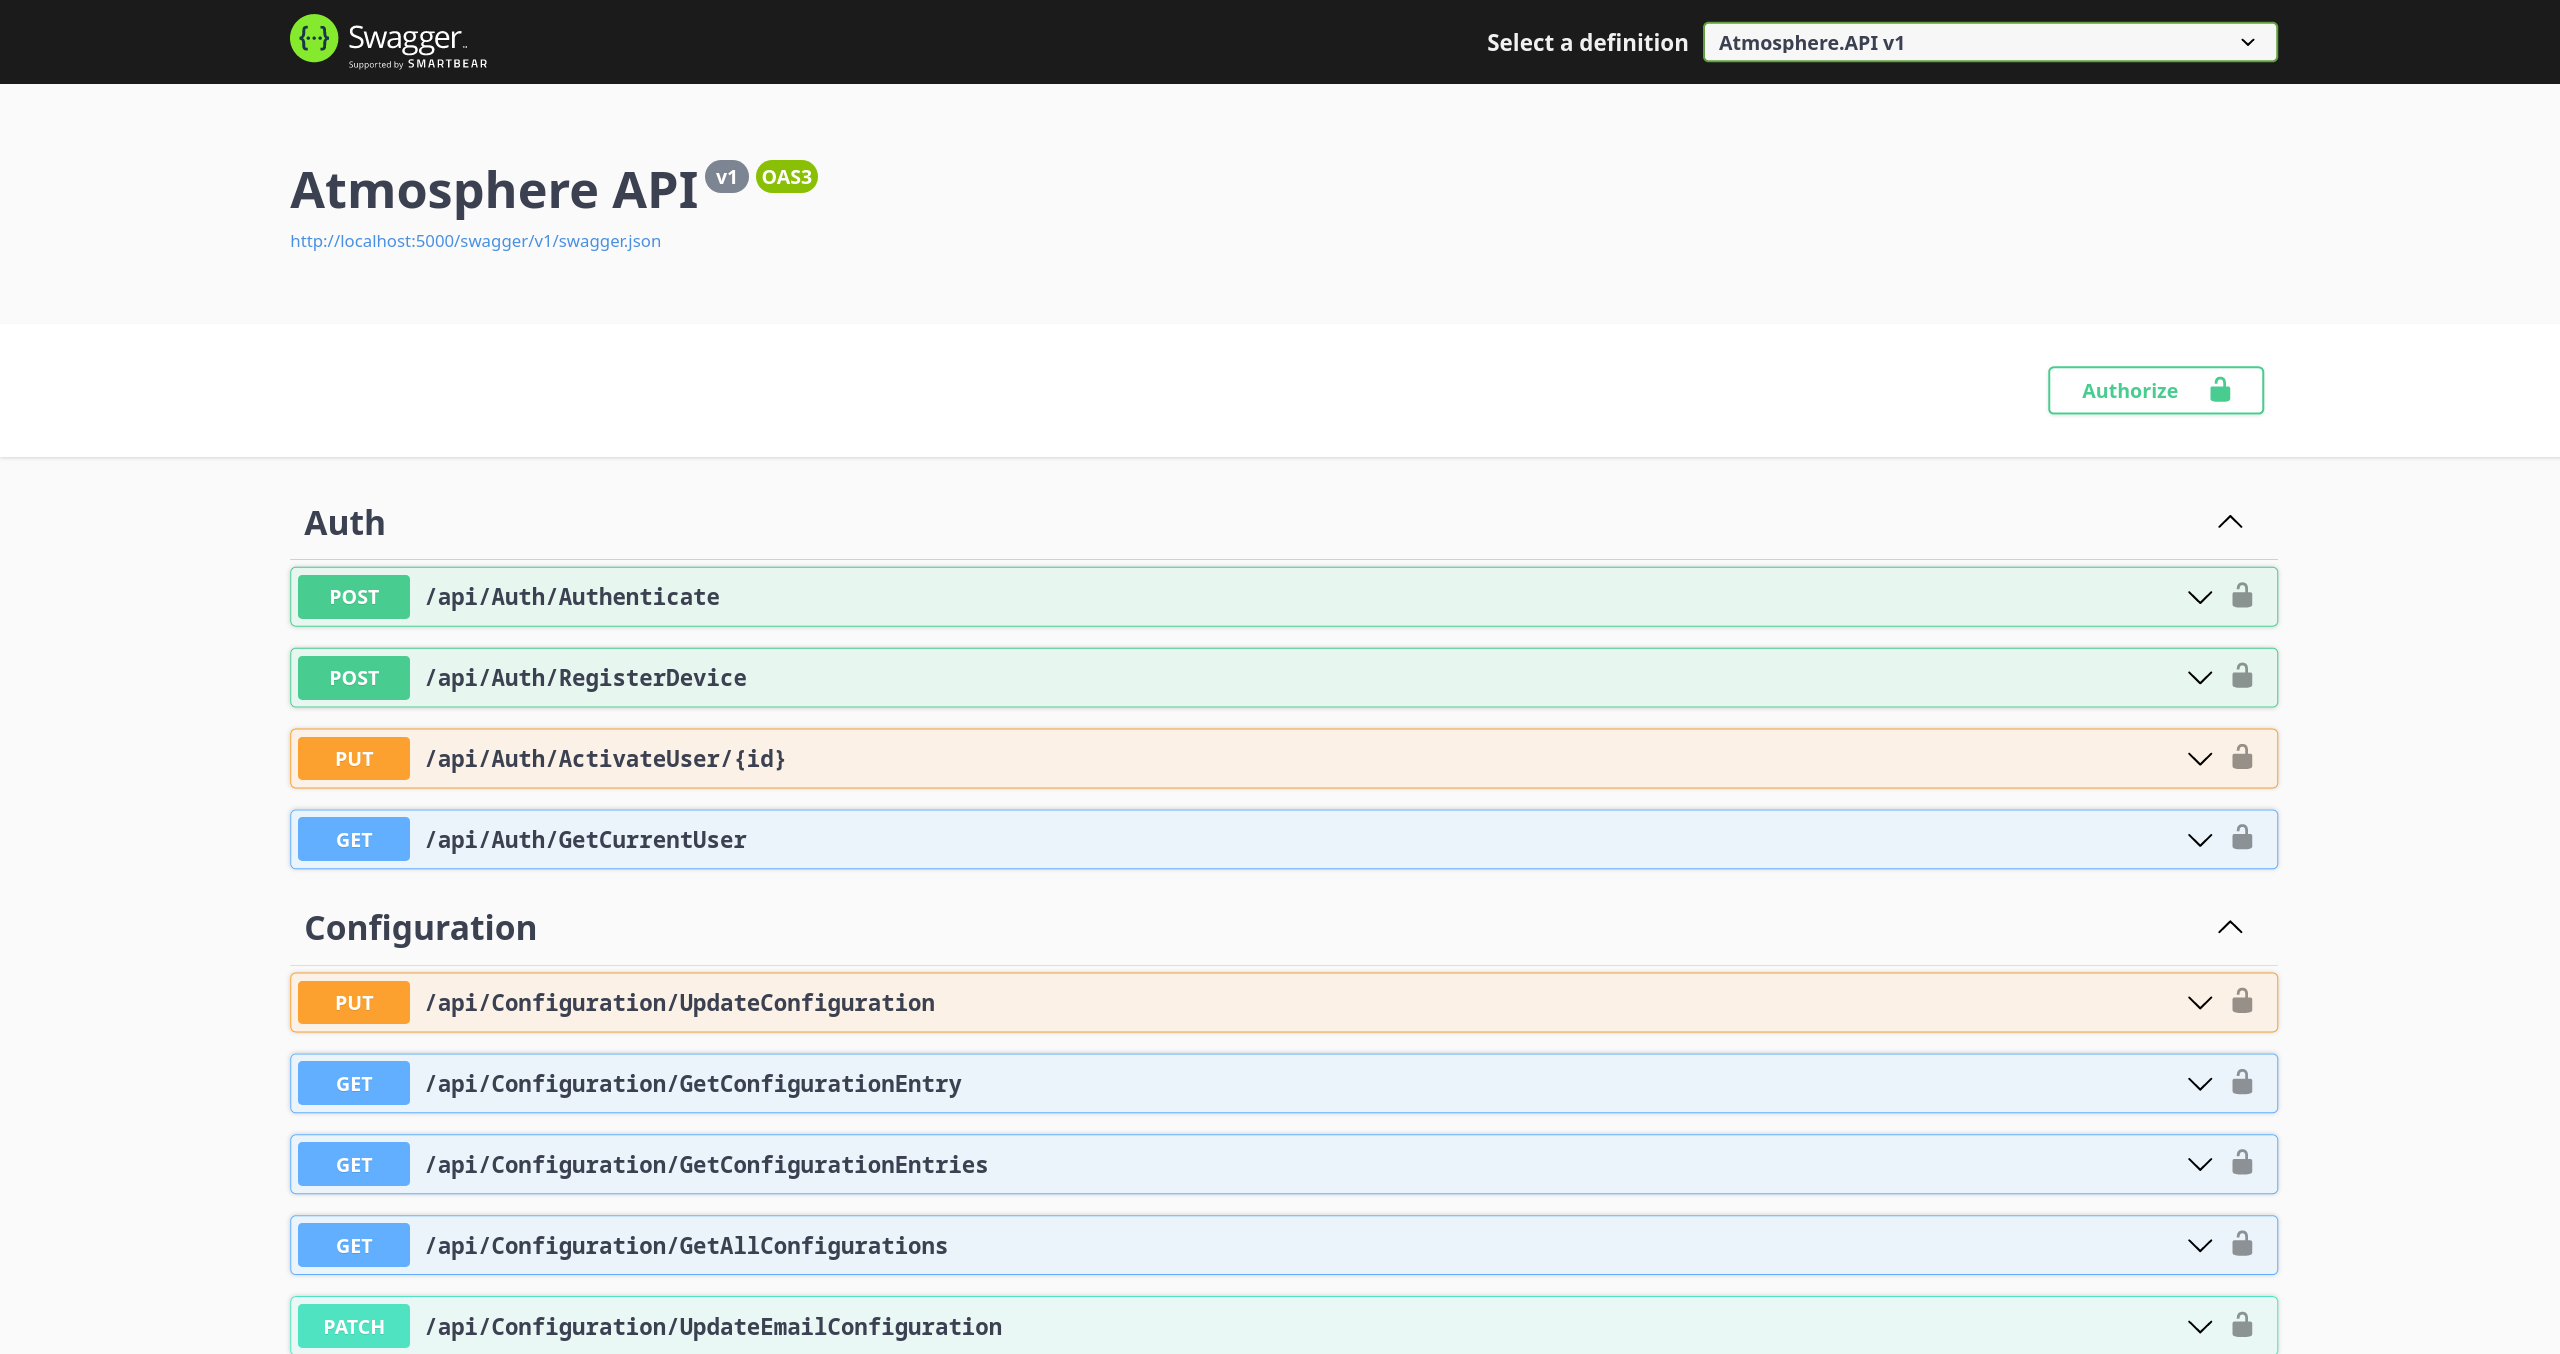
\includegraphics[width=\textwidth]{swagger}
  \caption{Intefejs swagger-ui}
  \label{swagger:interface}
\end{figure}
Kod wygenerowany na podstawie schematów wygenerowanych przez tą bibliotekę został następnie
wykorzystany zarówno w aplikacji klienckiej jak i urządzeniach pomiarowych.
Wykorzystano do tego oprogramowanie openapi-generator wspierające wiele języków
programowania oraz różnych bibliotek służących do komunikacji z użyciem protokołu HTTP.
Jest ono w stanie, na podstawie schematów OpenAPI, utworzyć klienta wraz z odpowiednimi
modelami jak również trzon aplikacji serwerowej oraz dokumentację. Pozwala również
na modyfikowanie wzorów generowanego kodu poprzez pliku mustache, za pomocą których
definiowana jest struktura wygenerowanych plików.

\section{Aplikacja kliencka}
Aplikacja kliencka powstała w celu ułatwienia dostępu do zasobów systemu.
Umożliwia ona na przedstawienie danych związanych z odczytami jak i konfigurację
aplikacji wykorzystując przyjazny użytkownikowi interfejs. W tym celu komunikuje
się ona z serwerem i na podstawie otrzymanych danych przedstawia je w formacie
czytelnym dla człowieka. 

\subsection{Architektura aplikacji}
Aplikacja kliencka dzieli się na komponenty oraz widoki z nich korzystające.
Do widoków należą podstrony tj.:
\begin{itemize}
  \item strona główna - zawiera listę odczytów w przypadku zalogowanego użytkownika
    lub przekierowanie do logowania w przeciwnym przypadku,
  \item strona z logowaniem - zawiera prosty formularz logowania,
  \item strona z ustawieniami - zawiera konfigurację aplikacji,
  \item strona z urządzeniami - zawiera listę urządzeń wraz z ich stanem połączenia,
  \item strona z użytkownikami - zawiera listę użytkowników oraz umożliwia na ich usunięcie.
\end{itemize}
Komponentami, które wykorzystywane są na każdej ze stron jest \textbf{UserContextProvider}
oraz \textbf{Nav}.
Zadaniem pierwszego z nich jest dostarczenie kontekstu użytkownika pozostałym komponentom i 
widokom. Drugi natomiast to pasek nawigacji zawierający odnośniki do pozostałych stron.
Zależnie od roli zalogowanego użytkownika wyświetla różne odnośniki.
Strona główna zawiera odniesienia do komponentu \textbf{ReadingList} odpowiedzialnego
za wyświetlanie listy odczytów oraz ich filtrowanie według daty.
Strona z ustawieniami natomiast używa komponentów \textbf{EmailConfig} zawierającego
ustawienia notyfikacji poprzez pocztę email oraz \textbf{ValidationRule} 
zawierającą ustawienia walidacji odczytów. Komponenty oraz strony, które
wymagają połączenia z aplikacją serwerową lub wykonują sprawdzanie danych
dodatkowo używają komponent toastów służący do wyświetlania informacji w okienku modalnym.

\subsection{Implementacja wybranych funkcjonalności}
Aby użytkownik nie musiał za każdym wejściem na stronę ponownie logować się
zastosowano przechowywanie tokena w pamięci lokalnej przeglądarki.
Gdy użytkownik ponownie odwiedza witrynę jeżeli był on wcześniej zalogowany
pobierany jest token z pamięci lokalnej, a następnie za jego pomocą pobierane
są jego dane. Na listingu \ref{lazy_token} przedstawiono ładowanie tokenu z pamięci
lokalnej, a \ref{load_user} przedstawia implementację wczytywania szczegółów użytkownika
z serwera wraz z komponentem \textbf{UserContextProvider}.
\begin{lstlisting}[caption={Wczytywanie tokenu z pamięci lokalnej},label={lazy_token},captionpos=b]
lazy_static! {
    pub static ref TOKEN: RwLock<Option<String>> = {
        if let Ok(token) = LocalStorage::get(TOKEN_KEY) {
            RwLock::new(Some(token))
        } else {
            RwLock::new(None)
        }
    };
}
\end{lstlisting}
Po zamontowaniu komponent \textbf{UserContextProvider} sprawdza czy istnieje w pamięci token,
a następnie w przypadku jego istnienia pobiera szczegóły użytkownika z serwera.
Jeżeli zapytanie powiodło się są one umieszczane w pamięci w przeciwnym przypadku
token jest z niej usuwany.
\begin{lstlisting}[caption={Implementacja komponentu UserContextProvider},label={load_user},captionpos=b]
#[function_component(UserContextProvider)]
pub fn user_context_provider(props: &Props) -> Html {
    let user_ctx = use_state(|| None);
    let current_user = use_async(async move { user::current().await });

    {
        let current_user = current_user.clone();
        use_mount(move || {
            if get_token().is_some() {
                current_user.run();
            }
        });
    }

    {
        let user_ctx = user_ctx.clone();
        use_effect_with_deps(
            move |current_user| {
                if let Some(user) = &current_user.data {
                    user_ctx.set(Some(user.clone()))
                }

                if let Some(err) = &current_user.error {
                    match err {
                        crate::error::Error::Unauthorized(_) => {
                            user_ctx.set(None);
                            set_token(None);
                        }
                        _ => {}
                    }
                }

                || ()
            },
            current_user.clone(),
        )
    }

    html! {
        <ContextProvider<UseStateHandle<Option<UserInfo>>> context={user_ctx} children={props.children.clone()} />
    }
}
\end{lstlisting}

Ze względu na limitację frameworku Yew implementacja okienek modalnych było 
znacznie łatwiejsze z wykorzystaniem języka TypeScript. Poprzez wykorzystanie
technologii wasm-bindgen zostały wygenerowane połączenia między językami co pozwoliło
na wykorzystanie kodu TypeScript w komponentach. Kod odpowiedzialny za
definicję interfejsu został przedstawiony na listingu \ref{js:bindings}, a
ich implementacja na listingu \ref{js:impl}.
\begin{lstlisting}[caption={Interfejs dla funkcjonalnosci notyfikacji oraz WebSocket},label={js:bindings},captionpos=b]
#[wasm_bindgen(module = "/src/js/notifications.ts")]
extern "C" {
    #[wasm_bindgen]
    pub fn notify(title: &str, body: &str);
    #[wasm_bindgen]
    pub fn show_error(text: &str);
    #[wasm_bindgen]
    pub fn set_send_ping_interval(ws: &web_sys::WebSocket, interval: u32);
    #[wasm_bindgen]
    pub fn set_on_close(ws: &web_sys::WebSocket);
}
\end{lstlisting}
Funkcje zaimplementowane w języku TypeScript tworzą okienka modalne z podanym tytułem oraz
wiadomością wykorzystując do tego funkcjonalność biblioteki Bootstrap. Tworzony jest
kontener na wiadomości mający indeks 9999 co oznacza, że będzie wyświetlany wyżej
od reszty komponentów i nie będzie przez nie zasłonięty oraz nie będzie ingerował w ich
wygląd. Dodatkowo w języku TypeScript zostały zaimplementowane niektóre funkcjonalności
związane z wykorzystaniem technologii WebSocket, takie jak wysyłanie wiadomości z ustalonym
interwałem oraz rozłączanie połączenia przy wyłączeniu okienka zawierającego stronę.
\begin{lstlisting}[caption={Implementacja funkcjonalnosci notyfikacji oraz WebSocket},label={js:impl},captionpos=b]
export function notify(title: string, msg: string) {
    var toast = build_toast(title, msg);
    var toast_container = document.getElementById('toast-container');
    if (toast_container === null) {
        toast_container = document.createElement('div');
        toast_container.id = 'toast-container';
        toast_container.classList.add('position-fixed', 'bottom-0', 'end-0', 'p-3');
        toast_container.style.zIndex = '9999';
        document.body.appendChild(toast_container);
    }

    toast_container.appendChild(toast);
    var toast_obj = new bootstrap.Toast(toast);
    toast_obj.show();
}

export function show_error(text: string) {
    notify('Error', text);
}

export function set_send_ping_interval(ws: WebSocket, interval: number) {
    setInterval(() => {
        ws.send('ping');
    }, interval);
}

export function set_on_close(ws: WebSocket) {
    window.onclose = () => {
        ws.close();
    };
}

function build_toast(title: string, msg: string) {
    var toast = document.createElement('div');
    toast.classList.add('toast');
    toast.setAttribute('role', 'alert');
    toast.setAttribute('aria-live', 'assertive');
    toast.setAttribute('aria-atomic', 'true');
    toast.innerHTML = `
        <div class="toast-header">
            <strong class="me-auto">${title}</strong>
            <button type="button" class="btn-close" data-bs-dismiss="toast" aria-label="Close"></button>
        </div>
        <div class="toast-body">
            ${msg}
        </div>
    `;

    return toast;
}
\end{lstlisting}

Zależnie od tego czy użytkownik jest zalogowany może on otrzymywać notyfikacje o przekroczeniu
wartości danych parametrów odczytów. Zostało to wykonane poprzez wykorzystanie połączenia 
WebSocket z serwerem, który w takich przypadkach wysyła wiadomość w formie JSON z polem
\textbf{type} o wartości \textit{notification}. Jeżeli użytkownik jest zalogowany i aplikacja
otrzyma taką wiadomość wykorzystywana jest wcześniej zaprezentowana funkcjonalność okienek modalnych,
aby wyświetlić informację zawartą w polu \textbf{data} wiadomości otrzymanej z serwera.
Kod odpowiedzialny za tą funkcjonalność został przedstawiony na lisitingu \ref{show_notif}.
\begin{lstlisting}[caption={Implementacja wyświetlania powiadomień},label={show_notif},captionpos=b]
use_effect_with_deps(
    move |_user| {
        if let Some(notification_ws) = &*notification_ws.clone() {
            let on_message = Closure::<dyn FnMut(_)>::new(move |e: MessageEvent| {
                let data = e.data().as_string().unwrap();
                if let Ok(notification) = serde_json::from_str::<NotificationPayload>(&data) {
                    if notification.r#type.to_lowercase() == "notification" {
                        bindings::notify("New notification", &notification.data.join(" "));
                    }
                }
            });
            notification_ws.set_onmessage(Some(on_message.as_ref().unchecked_ref()));
            on_message.forget();
            set_send_ping_interval(notification_ws, 20000);
            set_on_close(notification_ws);
        }
        || ()
    },
    (*user).clone(),
);
\end{lstlisting}


\section{Urządzenie pomiarowe}
Do wykonywania pomiarów wykorzystany został mikrokontroler Raspberry Pi Pico W.
W celu uproszczenia tworzenia oprogramowania użyto nieoficjalnej implementacji
środowiska Arduino dla płytek z rodziny RP2040. Udostępnia ona prosty
w obsłudze poziom abstrakcji, który umożliwia na wykorzystanie głównych
możliwości mikrokontrolera takich jak odczyty z portów czy możliwość połączenia
z siecią bezprzewodową Wi-Fi. Możliwe jest dzięki temu również korzystanie z
wielu bibliotek stworzonych przez społeczność, które znacznie ułatwiają implementację.
Przykładem takiego modułu jest OneWire - biblioteka dodająca obsługę sensorów 
wykorzystujących jedną linię danych jako magistralę.
Jej wykorzystanie umożliwiło wykorzystanie jednej linii danych do połączenia wielu 
sensorów tej samej klasy.

W celu ułatwienia komunikacji z serwerem wykorzystana została zmodyfikowana wersja
generatora cpp-tiny znajdująca się w oprogramowaniu openapi-generator wykorzystując
wygenerowaną dokumentację OpenAPI 3.0. 
Ze względu na różnice w implementacji frameworku Arduino, aby uzyskać poprawnie 
wygenerowany kod zostały dokonane zmiany do plików mustache odpowiadających za składnię
generowanego kodu. W pliku Service.h.mustache, będącej nagłówkiem klasy odpowiadającej za komunikację z serwerem
oraz odpowiadającym serwisem, w celu usprawnionej obsługi nagłówków
HTTP oraz ich przechowywaniu do wykonania zapytania dodano zmienną przechowujące te nagłówki.
Podobnie, aby dostosować się do zmienionej logiki w pliku Service.cpp.mustache zmodyfikowane
zostało zapisywanie nagłówków - zamiast przechowywać je w kliencie HTTP, gdzie byłyby usuwane podczas
rozpoczęcia zapytania, przechowywane są we wcześniej stworzonej zmiennej, a następnie są one
wstrzykiwane klientowi zaraz po rozpoczęciu zapytania oraz przed jego wysłaniem.
Podobnie w przypadku pustych odpowiedzi wygenerowany kod nie był ich w stanie obsłużyć,
ze względu na implementację klienta HTTP, co kończyło się dostępem do niezmapowanej pamięci. 
Aby to rozwiązać w funkcji odpowiedzialnej 
za pobieranie odpowiedzi dodano dodatkowe zabezpieczenie w postaci sprawdzenia
długości odpowiedzi, jeżeli wynosi -1 odpowiedź jest o nieznanej długości i całość przepisywana jest
do bufora z wykorzystaniem potoku, w przypadku 0 odpowiedź jest pusta, a przy wartościach większych od
0 tworzony jest bufor o tej długości.

\subsection{Architektura aplikacji}
Aplikacja udostępnia abstrakcyjną klasę \textbf{Sensor} zawierającą metody wymagane do 
podstawowej obsługi sensorów. W projekcie umieszczone zostały implementacje tej klasy
dla dwóch typów sensorów \textbf{OneWire} oraz \textbf{DHT}. Pierwszy z nich wykorzystuje
sensory Dallas Temperature, aby uzyskiwać wyniki temperatur. DHT natomiast jest w stanie
obsłużyć dwa sensory DHT11 oraz DHT22 obydwa posiadające możliwość pomiarów temperatury oraz
wilgotności powietrza. Implementacja została przedstawiona na diagramie klas \ref{diagram:sensors}.
\begin{figure}[h!]
  \centering
  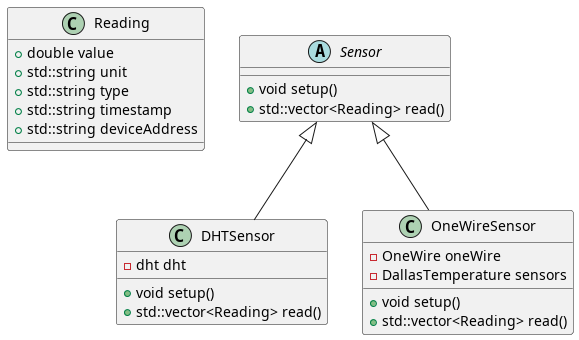
\includegraphics[width=\textwidth]{sensor_class}
  \caption{Diagram klas sensorów oraz odczytów}
  \label{diagram:sensors}
\end{figure}


\subsection{Implementacja wybranych funkcjonalności}
Podczas startu urządzenie łączy się z siecią Wi-Fi wcześniej zdefiniowaną przez użytkownika.
Jeżeli połączenie powiodło się następuje synchronizacja czasu z zewnętrznym serwerem NTP.
Zapewnia to spójność znaków czasu między urządzeniami w systemie, co wykorzystywane jest
przy procesowaniu pomiarów. Następnym krokiem jest inicjalizacja połączenia z serwerem.
Urządzenie najpierw próbuje przejść proces uwierzytelniania dostarczonym przez użytkownika
hasłem, jeżeli jest to pierwszy raz kiedy dane urządzenie łączy się z systemem tworzone jest
jemu nieaktywne konto, które następnie musi zostać zaakceptowane przez administratora.
Jeżeli wcześniejszy proces przebiegł z powodzeniem urządzenie kontynuuje do połączenia
z odpowiednim kanałem WebSocket po czym przechodzi do stanu normalnej operacji.
Aby zapewnić synchronizację z serwerem oraz dostęp do statusu połączenia wykorzystano
technologię WebSocket. Kod inicjalizacji połączenia został zaprezentowany na lisitingu
\ref{sconn:init}.
\begin{lstlisting}[language={C++},caption={Utworzenie konta i połączenie z serwerem},label={sconn:init},captionpos=b]
void init_server_connection() {
  Serial.println("Setup api");
  const char *mac = WiFi.macAddress().c_str();
  Tiny::Authenticate authPayload;
  authPayload.setUsername(mac);
  authPayload.setPassword(PASSWD);
  auto response = authApi.apiAuthAuthenticatePost(authPayload);
  if (response.code != 200) {
    Serial.println("Device not registered. Registering...");
    Tiny::RegisterDevice registerDevicePayload;
    registerDevicePayload.setIdentifier(authPayload.getUsername());
    registerDevicePayload.setUsername(authPayload.getUsername());
    registerDevicePayload.setPassword(PASSWD);
    auto response = authApi.apiAuthRegisterDevicePost(registerDevicePayload);
    if (response.code != 200) {
      Serial.printf("Error: %d\r\n", response.code);
      return;
    }

    auto response2 = authApi.apiAuthAuthenticatePost(authPayload);
    if (response2.code != 200) {
      Serial.printf("Error: %d\r\n", response2.code);
      return;
    }

    token = response2.obj.getToken();
  } else {
    token = response.obj.getToken();
  }

  Serial.println("Setup websocket");
  std::string wsPath = BASE_WS_PATH + token;
  webSocket.begin(API_HOST, HOST_PORT, wsPath.c_str(), "");
  webSocket.onEvent(onEvent);
  webSocket.setReconnectInterval(5000);
}
\end{lstlisting}
Urządzenie łączy się z odpowiednim gniazdem, a następnie co 30
sekund wysyła wiadomość z zawartością "ping" i oczekuje na odpowiedź "pong" od serwera.
Jeżeli nie otrzyma takiej wiadomości uznaje, że połączenie zostało zerwane, więc zamyka je
i po upływie 5 sekund próbuje utworzyć ponowną komunikację. Dzieje się to aż do momentu przywrócenia
połączenia po czym urządzenie powraca do normalnego trybu operacji odczytywania oraz
przesyłania danych z sensorów.

Urządzenie pomiarowe, podczas normalnej operacji, dokonuje pomiarów z podłączonych sensorów, 
a następnie przetwarza je i w odpowiednim formacie wysyła na serwer. Odbywa się to poprzez
wykorzystanie metody POST jednego z kontrolerów. Dane pomiaru zawierają takie informacje jak
data i czas wykonania, wartość, jednostka oraz typ pomiaru. Do autoryzacji tego zapytania
wykorzystywany jest wcześniej wygenerowany token JWT. Następnie urządzenie odczekuje wcześniej
skonfigurowaną ilość czasu przed następnym pomiarem. Jest ona obliczana jako różnica czasu, który
został spędzony na aktualnym przejściu, a ustalonym przez użytkownika okresem. Jeżeli jest ona
większa od zera urządzenie wyczekuje wyliczony przedział czasu, a następnie kontynuuje pracę.
Implementacja tego procesu została zaprezentowana na listingu \ref{sensor:loop}.
\begin{lstlisting}[language={C++},caption={Główna pętla urządzenia pomiarowego},label={sensor:loop},captionpos=b]
static auto end = 0;
static auto diff = 0;
void loop() {
  while (!webSocket.isConnected()) {
    webSocket.loop();
  }

  auto begin = millis();
  webSocket.loop();

  if (last_ping > ping_interval) {
    if (webSocket.isConnected())
      webSocket.sendTXT("ping");
    last_ping = 0;
  }

  if (diff >= send_interval) {
    diff = 0;
    std::vector<Reading> readings;
    for (auto sensor : sensors) {
      auto sensorReadings = sensor->read();
      readings.insert(readings.end(), sensorReadings.begin(),
                      sensorReadings.end());
    }

    auto body = convert(readings);
    auto auth = "Bearer " + token;
    readingApi.addHeader("Authorization", auth);
    auto response = readingApi.apiReadingCreateReadingsPost(body);
  }

  end = millis();
  last_ping += end - begin;
  diff += end - begin;
}
\end{lstlisting}

Do wykonywania pomiarów temperatur wykorzystano sensor DS1820B20. To urządzenie
wykorzystuje pojedyncze połączenie z kontrolerem umożliwiające na łączność
z wieloma sensorami na jednej linii danych. Ta funkcjonalność została wykorzystana
w implementacji i wartości pobierane są ze wszystkich sensorów podłączonych do tej
linii. Implementacja pobierania danych z sensorów została zaprezentowana na listingu 
\ref{onewire:impl}.
\begin{lstlisting}[language={C++},caption={Implementacja systemu OneWire},label={onewire:impl},captionpos=b]
std::vector<Reading> OneWireSensor::read() {
  std::vector<Reading> readings;
  sensors.requestTemperatures();
  uint8_t deviceCount = sensors.getDeviceCount();
  float value = 0;
  for (uint8_t i = 0; i < deviceCount; i++) {
    DeviceAddress deviceAddress;
    if (sensors.getAddress(deviceAddress, i)) {
      std::stringstream stream;
      for (int i = 0; i < 8; ++i) {
        stream << std::setfill('0') << std::setw(2) << std::hex
               << (uint)deviceAddress[i];
      }
      float temp = sensors.getTempC(deviceAddress);
      value += temp;

      auto now = time(nullptr);
      struct tm timeinfo;
      gmtime_r(&now, &timeinfo);
      char buf[sizeof("2011-10-08T07:07:09Z")];
      strftime(buf, sizeof(buf), "%FT%TZ", &timeinfo);
      readings.push_back(Reading{temp, "C", "temperature", stream.str(), buf});
    }
  }

  return readings;
}
\end{lstlisting}

\chapter{Podsumowanie}
Wytworzona aplikacja spełnia pierwotne założenia pracy. Umożliwia ona na 
wykorzystanie funkcjonalności tj. zbieranie oraz odczyt parametrów środowiska,
przeglądanie danych historycznych oraz powiadamianie użytkownika o niespodziewanych
sytuacjach. Dodatkowo system posiada możliwość uwierzytelniania oraz autoryzacji 
użytkowników oraz urządzeń w celu zapewnienia bezpieczeństwa przechowywanych danych.
Dzięki zastosowanym wzorcom projektowym oraz modularnej architekturze aplikacja
jest podatna na rozwój w przyszłości o nowe funkcjonalności oraz rozszerzenie
aktualnie istniejących rozwiązań. Możliwym wektorem dalszego rozwoju jest
uproszczenie interfejsu oraz procesu wprowadzania w celu zwiększenia dostępności
dla większej audiencji. Aktualna implementacja obiera za cel użytkowników zaznajomionych
z systemami komputerowymi oraz wymaga od nich dodatkowej wiedzy, np. przy konfiguracji
urządzeń pomiarowych. 

Ze względu na obszerność problemu trudnym jest wytworzenie systemu odpowiadającego
każdej sytuacji, jednak powtarzająca się funkcjonalność umożliwiła wytworzenie
solidnej bazy oprogramowania, które może zostać rozwinięte do szczególnych zastosowań.


\nocite{*} %wszystkie wpisy w bibliografi
\Urlmuskip=0mu plus 1mu\relax
\def\UrlBreaks{\do\/\do-}
\bibliographystyle{plain} %{latex8} posortowane wzgledem wystepowania
\bibliography{bibliografia}%
\listoffigures

%\biblioteka{tak} % tak/nie
\end{document}
